% =============================================================================
% EpiForecast-MX — Documentación Técnica: Sistema de Visualización Tableau
% Equipo 01 — Maestría en Inteligencia Artificial Aplicada (MNA)
% Tecnológico de Monterrey x Instituto Mexicano del Seguro Social
% =============================================================================
\documentclass[12pt, letterpaper]{article}

% -- Paquetes ----------------------------------------------------------------
\usepackage[utf8]{inputenc}
\usepackage[T1]{fontenc}
\usepackage{babel}
\usepackage{geometry}
\geometry{letterpaper, margin=2.5cm, top=3cm, bottom=2.5cm}
\setlength{\headheight}{14pt}
\setlength{\emergencystretch}{3em}
\usepackage{graphicx}
\graphicspath{{FigurasConclu/}{FigurasTableau/}}
\usepackage{float}
\usepackage{booktabs}
\usepackage{tabularx}
\usepackage{longtable}
\usepackage{multirow}
\usepackage{xcolor}
\usepackage{colortbl}
\usepackage{fancyhdr}
\usepackage{titlesec}
\usepackage{enumitem}
\usepackage{amsmath, amssymb}
\usepackage{caption}
\usepackage{subcaption}
\usepackage[most]{tcolorbox}
\usepackage{pifont}
\usepackage{parskip}
\usepackage{setspace}
\usepackage{array}
\usepackage[bottom]{footmisc}
\usepackage{xurl}
\usepackage[breaklinks=true]{hyperref}
\usepackage{tikz}
\usetikzlibrary{arrows.meta, positioning, shapes.geometric, fit, calc,
                decorations.pathreplacing, shadows.blur, colorbrewer, babel}
\usepackage{pdflscape}
\usepackage{multicol}

% -- Colores institucionales -------------------------------------------------
\definecolor{burgundy}{HTML}{9B2242}
\definecolor{darkburgundy}{HTML}{6F1D46}
\definecolor{teal}{HTML}{00524E}
\definecolor{darkteal}{HTML}{173F35}
\definecolor{gold}{HTML}{B58500}
\definecolor{coolgray}{HTML}{97999B}
\definecolor{imssblue}{HTML}{003A70}
\definecolor{cream}{HTML}{F5EDE0}
\definecolor{lightgreen}{HTML}{E6F4EA}
\definecolor{lightyellow}{HTML}{FEF7E0}
\definecolor{lightred}{HTML}{FDE8E8}
% Off-palette
\definecolor{slateborder}{HTML}{4A5568}
\definecolor{slatelight}{HTML}{EDF2F7}
\definecolor{burntborder}{HTML}{C05621}
\definecolor{burntlight}{HTML}{FEEBC8}

% -- Hyperref ----------------------------------------------------------------
\hypersetup{
    colorlinks=true, linkcolor=teal, citecolor=burgundy, urlcolor=imssblue,
    bookmarksopen=true,
    pdftitle={EpiForecast-MX | Sistema de Visualización Tableau},
    pdfauthor={Equipo 01 | MNA Tec de Monterrey},
}

% -- Captions ----------------------------------------------------------------
\captionsetup{font={small,color=coolgray}, labelfont={bf,color=coolgray},
              justification=centering}

% -- Headers y footers -------------------------------------------------------
\pagestyle{fancy}
\fancyhf{}
\fancyhead[L]{\small\textcolor{coolgray}{EpiForecast-MX | Sistema de Visualización Tableau}}
\fancyhead[R]{\small\textcolor{coolgray}{Equipo 01 | MNA | Tec de Monterrey}}
\fancyfoot[C]{\thepage}
\fancyfoot[R]{\small\textcolor{coolgray}{Marzo 2026}}
\renewcommand{\headrulewidth}{0.4pt}
\renewcommand{\footrulewidth}{0.2pt}

% -- Títulos -----------------------------------------------------------------
\titleformat{\section}
  {\Large\bfseries\color{teal}}{\thesection.}{0.5em}{}
  [\vspace{-0.5em}\textcolor{teal}{\rule{\textwidth}{1pt}}]
\titleformat{\subsection}
  {\large\bfseries\color{burgundy}}{\thesubsection}{0.5em}{}
\titleformat{\subsubsection}
  {\normalsize\bfseries\color{darkteal}}{\thesubsubsection}{0.5em}{}

% -- Cajas de callout --------------------------------------------------------
\newtcolorbox{insightbox}[1][]{
  colback=lightgreen, colframe=teal, boxrule=0pt, leftrule=4pt, arc=2pt,
  fonttitle=\bfseries, title=#1,
  before upper={\setlength{\emergencystretch}{5em}}}
\newtcolorbox{warningbox}[1][]{
  colback=lightyellow, colframe=gold, boxrule=0pt, leftrule=4pt, arc=2pt,
  fonttitle=\bfseries, title=#1,
  before upper={\setlength{\emergencystretch}{5em}}}
\newtcolorbox{criticalbox}[1][]{
  colback=lightred, colframe=burgundy, boxrule=0pt, leftrule=4pt, arc=2pt,
  fonttitle=\bfseries, title=#1,
  before upper={\setlength{\emergencystretch}{5em}}}

% -- Comandos personalizados -------------------------------------------------
\newcommand{\smape}{\textnormal{\textsc{smape}}}
\newcommand{\mase}{\textnormal{\textsc{mase}}}
\newcommand{\rmse}{\textnormal{\textsc{rmse}}}
\newcommand{\mae}{\textnormal{\textsc{mae}}}
\newcommand{\mape}{\textnormal{\textsc{mape}}}
\newcommand{\imss}{\textnormal{\textsc{imss}}}
\newcommand{\tabref}[1]{Tabla~\ref{#1}}
\newcommand{\figref}[1]{Figura~\ref{#1}}
\newcommand{\secref}[1]{Sección~\ref{#1}}
\newcommand{\sepsection}{\vspace{0.5cm}\noindent\textcolor{coolgray}
  {\rule{\textwidth}{0.3pt}}\vspace{0.3cm}}

% -- ERD styles --------------------------------------------------------------
\pgfdeclarelayer{background}
\pgfsetlayers{background,main}
\newlength{\rowh}  \setlength{\rowh}{0.52cm}
\newlength{\tabw}  \setlength{\tabw}{5.4cm}
\newlength{\hdrh}  \setlength{\hdrh}{0.62cm}
\tikzset{
  dbheader/.style={rectangle, draw=#1, fill=#1,
    minimum width=\tabw, minimum height=\hdrh, anchor=north, align=center,
    font=\sffamily\bfseries\small\color{white}, inner sep=0pt},
  dbkeyrow/.style={rectangle, draw=#1!30, fill=#1!06,
    minimum width=\tabw, minimum height=\rowh,
    text width=\dimexpr\tabw-12pt\relax,
    anchor=north, align=left, font=\sffamily\small\bfseries\color{#1},
    inner xsep=6pt, inner ysep=0pt},
  dbdatarow/.style={rectangle, draw=coolgray!25, fill=white,
    minimum width=\tabw, minimum height=\rowh,
    text width=\dimexpr\tabw-12pt\relax,
    anchor=north, align=left, font=\sffamily\small\color{black!70},
    inner xsep=6pt, inner ysep=0pt},
  conn/.style={draw=coolgray, thick, shorten >=2pt, shorten <=2pt},
  joinlabel/.style={rectangle, fill=white, draw=coolgray!40,
    font=\sffamily\scriptsize\color{coolgray!80},
    inner sep=3pt, rounded corners=2pt},
}
\newcommand{\erdpk}{\textcolor{gold}{\textbf{[PK]}}}
\newcommand{\erdfk}{\textcolor{imssblue}{\textbf{[FK]}}}
\newcommand{\keyicon}{{\small$\bullet$}\ }
\newcommand{\dataicon}{{\small\textcolor{coolgray}{$\circ$}}\ }

% =============================================================================
\begin{document}

% =============================================================================
% PORTADA
% =============================================================================
\begin{titlepage}
\begin{center}
\vspace*{0.5cm}

\includegraphics[height=2cm]{logo_tec.png}\hspace{2cm}

\includegraphics[height=2.5cm]{logo_imss.png}\\[0.5cm]
{\small Instituto Tecnológico y de Estudios Superiores de Monterrey}\\[0.1cm]
{\small Maestría en Inteligencia Artificial Aplicada (MNA)}\\[0.5cm]
\textcolor{teal}{\rule{\textwidth}{2pt}}\\[0.4cm]
{\Huge\bfseries\textcolor{teal}{EpiForecast-MX}}\\[0.2cm]
{\LARGE\textcolor{burgundy}{Sistema de Visualización Epidemiológica}}\\[0.2cm]
{\large\textcolor{darkteal}{Documentación Técnica — Tableau Public}}\\[0.3cm]
\textcolor{teal}{\rule{\textwidth}{2pt}}\\[0.8cm]
{\large\textit{Arquitectura de datos, pipeline de generación del dataset,\\
modelo relacional, diseño del workbook y automatización\\
de la publicación en \texttt{viz\_epiforecastmx.twb}}}\\[1.2cm]
{\large\textbf{Materia:} Proyecto Integrador | TC5035.10}\\[0.5cm]
\begin{tabular}{ll}
\textbf{Asesora:}     & Dra.\ Grettel Barceló Alonso \\
\textbf{Director MNA:}& Dr.\ Luis Eduardo Falcón Morales \\
\textbf{Profesora:}   & Mtra.\ Verónica Sandra Guzmán de Valle \\
\textbf{IMSS:}        & Dra.\ Ruth Pérez-Hernández (Líder de Proyecto) \\
                      & Dra.\ Lina Díaz Castro (Investigadora en Psiquiatría) \\
\end{tabular}\\[1cm]
\textbf{\Large Equipo 01}\\[0.4cm]
\begin{tabular}{lll}
\textbf{Javier A. Rebull Saucedo} & A01795838 & Sr.\ Assoc.\ Dev., Santander Bank US \\
\textbf{Juan Carlos Pérez Nava}   & A01795941 & Head of Area, IMSS \\
\textbf{Luis G. Sánchez Salazar}  & A01232963 & Sr.\ Controls Engineer, Tesla \\
\end{tabular}\\[1.0cm]
{\large Marzo 2026}
\end{center}
\end{titlepage}

% =============================================================================
% TABLA DE CONTENIDOS
% =============================================================================
\newpage
\tableofcontents
\newpage
\listoffigures
\listoftables
\newpage

% =============================================================================
% 1. VISIÓN GENERAL DEL SISTEMA
% =============================================================================
\section{Visión General del Sistema}\label{sec:vision}

El archivo \texttt{viz\_epiforecastmx.twb} constituye el libro de trabajo de Tableau que implementa el sistema de visualización del proyecto \textbf{EpiForecast-MX}. Su propósito es integrar en una sola plataforma interactiva tres dimensiones analíticas complementarias que, en conjunto, permiten transformar datos epidemiológicos complejos en información accionable para tomadores de decisiones clínicas y administrativas del {\imss}.

\begin{table}[H]
\centering
\caption{Dimensiones analíticas del sistema de visualización}
\label{tab:dimensiones}
\small
\begin{tabularx}{\textwidth}{>{\bfseries}l X}
\toprule
\textbf{Dimensión} & \textbf{Descripción} \\
\midrule
Exploración epidemiológica & Análisis descriptivo de los datos históricos provenientes del Sistema Nacional de Vigilancia Epidemiológica (\textsc{sinave}), con desagregación por entidad federativa, padecimiento y género. \\
Predicción epidemiológica  & Visualización de pronósticos generados por modelos de \textit{forecasting} entrenados para las 333 combinaciones geográficas y epidemiológicas de producción, con horizontes de hasta 52 semanas. \\
Monitoreo del sistema      & Seguimiento del desempeño de los modelos de predicción, distribución de algoritmos en producción y cobertura del sistema de pronóstico. \\
\bottomrule
\end{tabularx}
\end{table}

El dashboard permite analizar información epidemiológica combinada con variables demográficas y territoriales del \textsc{inegi} (2024), facilitando la interpretación de patrones espaciales y temporales de la incidencia de tres padecimientos de la Clasificación Internacional de Enfermedades: Depresión (F32), Parkinson (G20) y Alzheimer (G30).

\subsection{Usuarios potenciales}

El sistema está diseñado para tres perfiles de usuario diferenciados:

\begin{itemize}[noitemsep]
    \item \textbf{Epidemiólogos delegacionales del {\imss}}: interpretación de pronósticos para planificación de insumos y recursos humanos.
    \item \textbf{Directivos y tomadores de decisiones}: seguimiento de KPIs del sistema y tendencias nacionales.
    \item \textbf{Equipo técnico}: monitoreo del desempeño de los 333 modelos de producción, validación semanal y detección de degradación.
\end{itemize}

El workbook está publicado en Tableau Public y accesible desde \url{https://proyectointegrador.org/epidashboard}, sin requerir instalación de software.

\newpage
% =============================================================================
% 2. ARQUITECTURA GENERAL DEL SISTEMA
% =============================================================================
\section{Arquitectura General del Sistema}\label{sec:arquitectura}

La \figref{fig:flujo_tableau} presenta el flujo completo de información del sistema, desde las fuentes de datos primarias hasta las visualizaciones embebidas en el sitio web del proyecto.

\begin{figure}[H]
\centering
\resizebox{0.80\textwidth}{!}{%
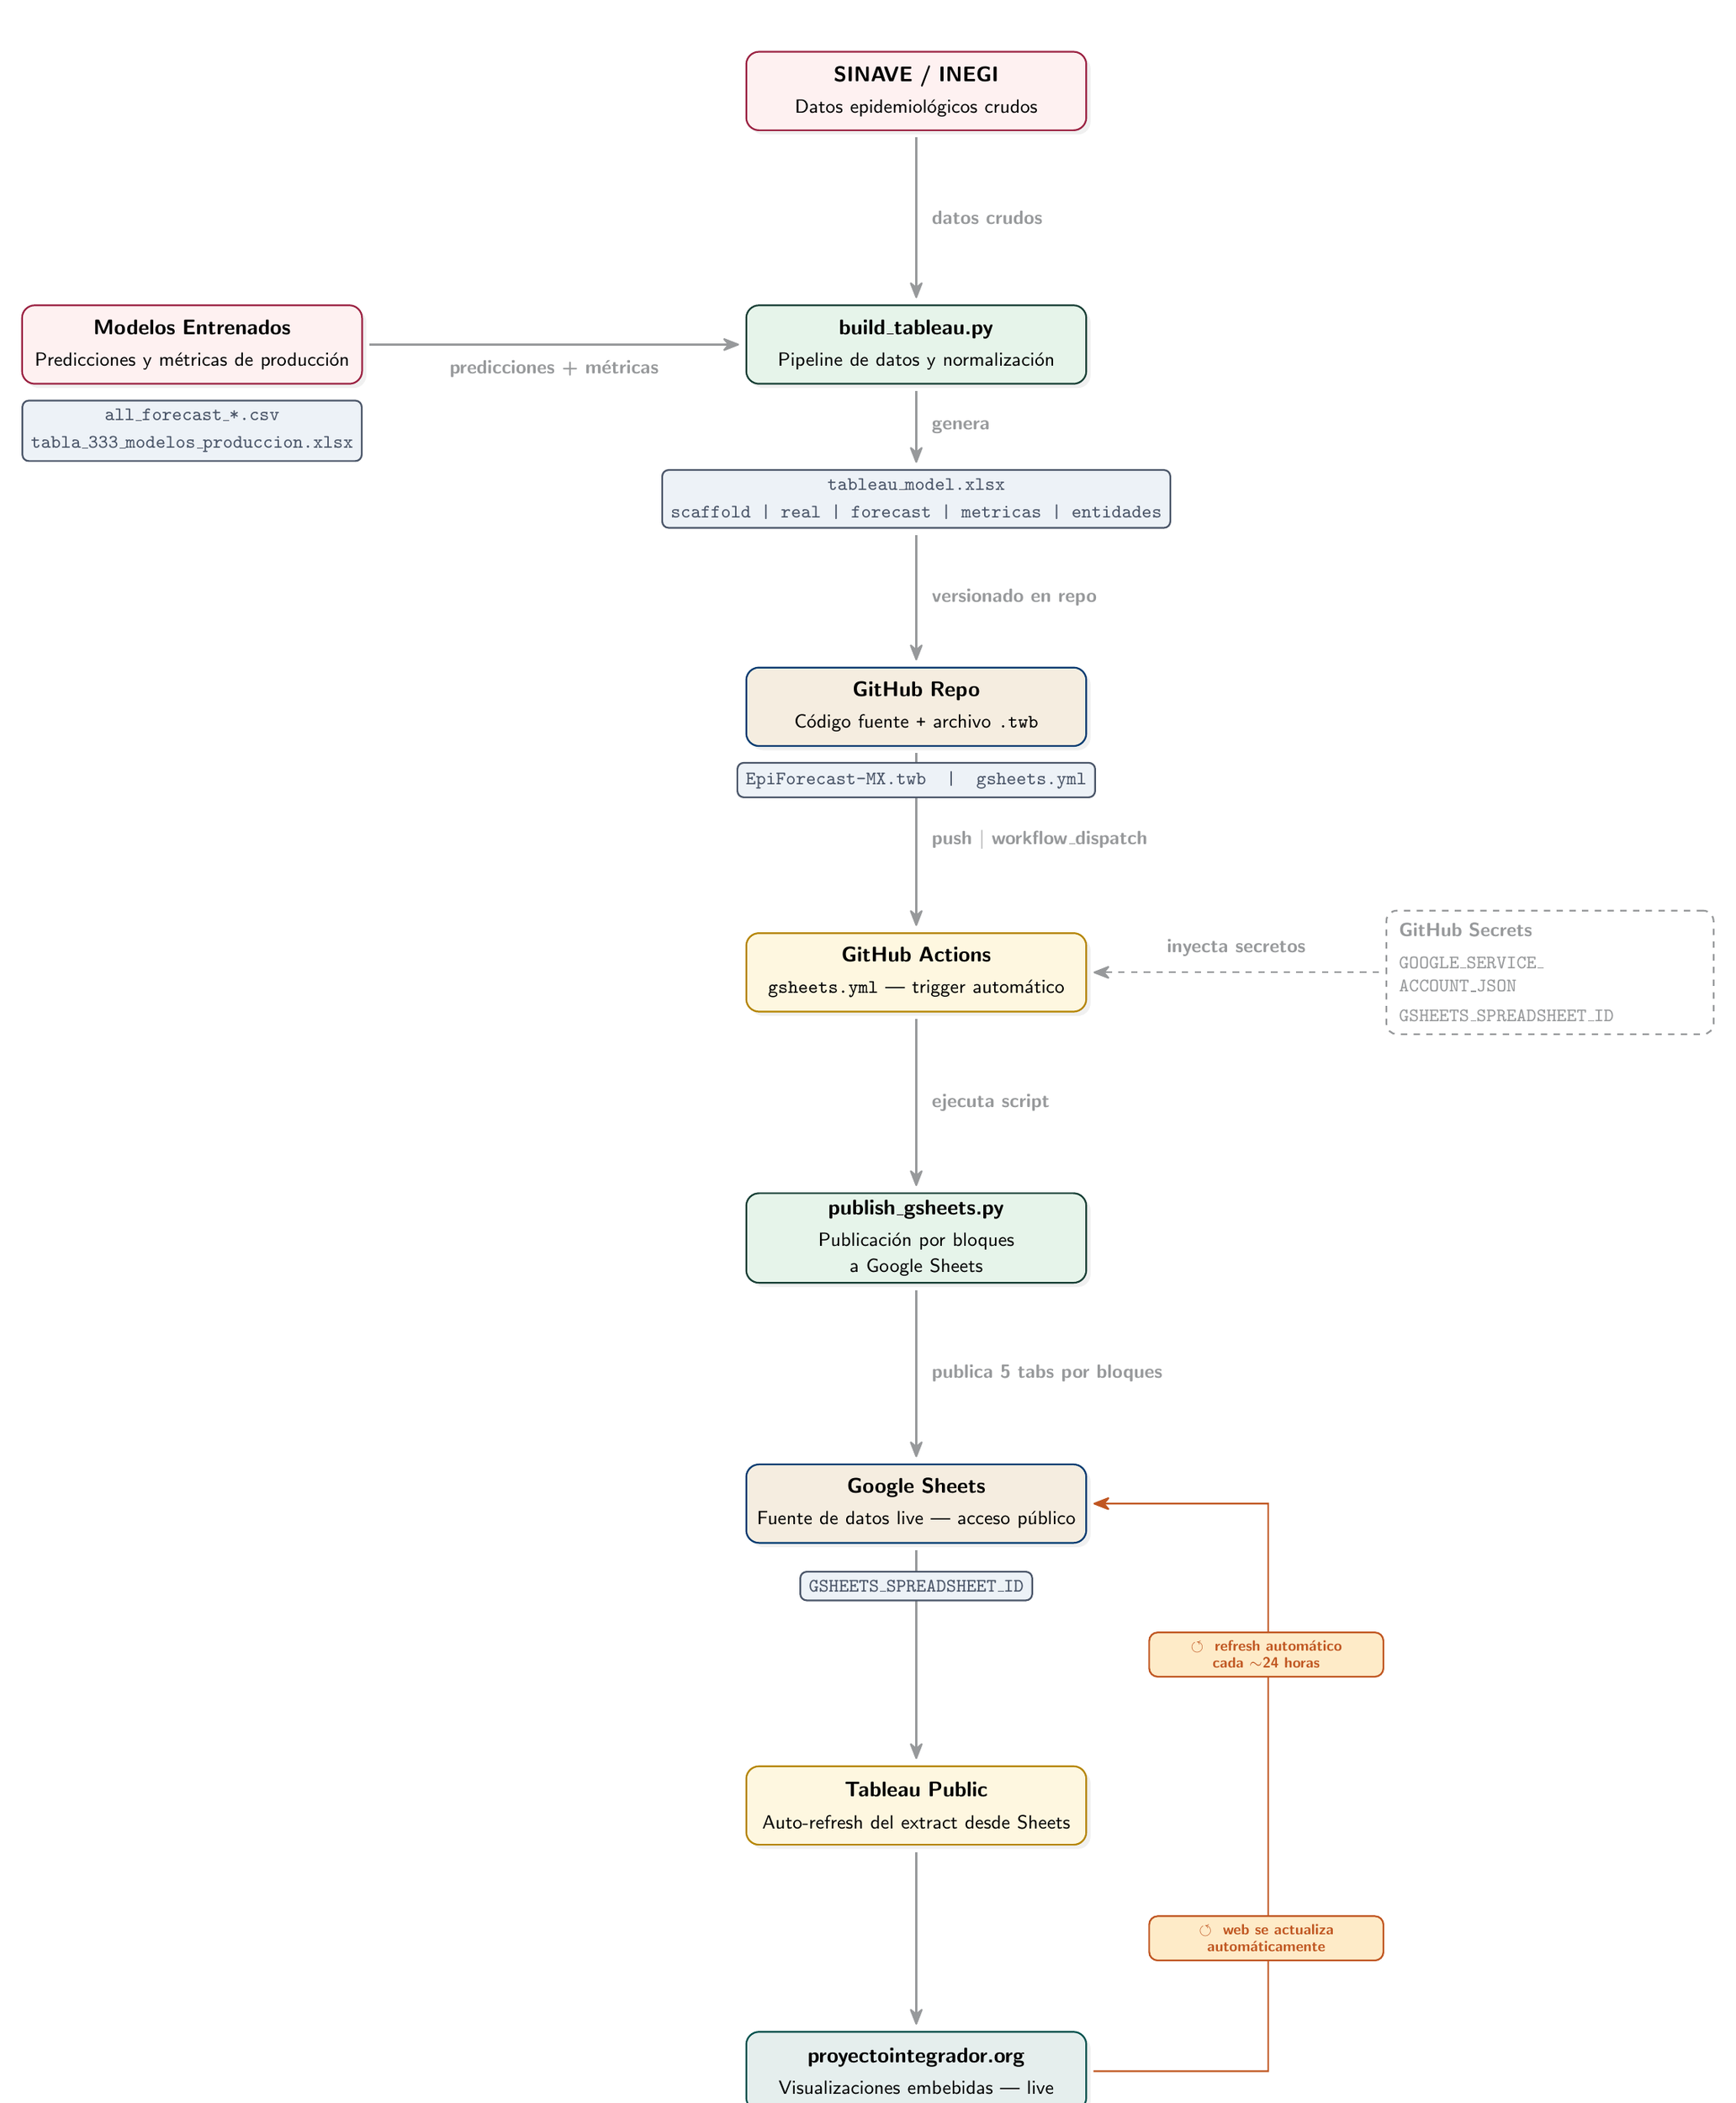
\begin{tikzpicture}[
    base/.style={thick, rounded corners=6pt,
      minimum width=5.6cm, minimum height=1.3cm, text width=5.4cm,
      align=center, font=\sffamily\normalsize,
      drop shadow={opacity=0.12, shadow xshift=2pt, shadow yshift=-2pt}},
    source/.style ={base, draw=burgundy, fill=lightred!60},
    script/.style ={base, draw=darkteal, fill=lightgreen},
    store/.style  ={base, draw=imssblue, fill=cream},
    cloud/.style  ={base, draw=gold,     fill=lightyellow},
    output/.style ={base, draw=teal,     fill=teal!10},
    filebadge/.style={font=\sffamily\small\ttfamily\color{slateborder},
      fill=slatelight, draw=slateborder,
      inner sep=4pt, rounded corners=3pt, thick, align=center},
    secretbadge/.style={font=\sffamily\small\color{coolgray},
      fill=white, draw=coolgray, dashed,
      inner sep=6pt, rounded corners=5pt, thick,
      align=left, text width=5.0cm},
    autobadge/.style={font=\sffamily\scriptsize\bfseries\color{burntborder},
      fill=burntlight, draw=burntborder,
      inner sep=4pt, rounded corners=4pt, thick,
      align=center, text width=3.6cm},
    edgelabel/.style={font=\sffamily\small\bfseries\color{coolgray},
      fill=white, inner sep=3pt, rounded corners=4pt},
    arrow/.style={-{Stealth[round, length=9pt, width=7pt]},
      thick, color=coolgray, shorten >=3pt, shorten <=3pt},
    arrowdashed/.style={-{Stealth[round, length=9pt, width=7pt]},
      thick, color=coolgray, dashed, shorten >=3pt, shorten <=3pt},
    looparrow/.style={-{Stealth[round, length=9pt, width=7pt]},
      thick, color=burntborder, shorten >=3pt, shorten <=3pt},
]
% Nodes
\node[source] (sinave) at (0, 0)
    {\textbf{SINAVE / INEGI}\\[1mm]\small Datos epidemiológicos crudos};
\node[source] (modelos) at (-12.0, -4.2)
    {\textbf{Modelos Entrenados}\\[1mm]\small Predicciones y métricas de producción};
\node[filebadge, below=0.25cm of modelos, align=center] (modelosbadge)
    {\texttt{all\_forecast\_*.csv}\\[2pt]\texttt{tabla\_333\_modelos\_produccion.xlsx}};
\node[script] (build) at (0, -4.2)
    {\textbf{build\_tableau.py}\\[1mm]\small Pipeline de datos y normalización};
\node[filebadge, below=1.4cm of build, align=center] (xlsxbadge)
    {\texttt{tableau\_model.xlsx}\\[2pt]
     \texttt{scaffold\ |\ real\ |\ forecast\ |\ metricas\ |\ entidades}};
\node[store] (github) at (0, -10.2)
    {\textbf{GitHub Repo}\\[1mm]\small Código fuente \texttt{+} archivo \texttt{.twb}};
\node[filebadge, below=0.25cm of github] (gitbadge)
    {\texttt{EpiForecast-MX.twb\ \ |\ \ gsheets.yml}};
\node[cloud] (gha) at (0, -14.6)
    {\textbf{GitHub Actions}\\[1mm]\small \texttt{gsheets.yml} — trigger automático};
\node[script] (publish) at (0, -19.0)
    {\textbf{publish\_gsheets.py}\\[1mm]\small Publicación por bloques a Google Sheets};
\node[store] (gsheets) at (0, -23.4)
    {\textbf{Google Sheets}\\[1mm]\small Fuente de datos live — acceso público};
\node[filebadge, below=0.45cm of gsheets] (sheetbadge)
    {\texttt{GSHEETS\_SPREADSHEET\_ID}};
\node[cloud] (tableau) at (0, -28.4)
    {\textbf{Tableau Public}\\[1mm]\small Auto-refresh del extract desde Sheets};
\node[output] (website) at (0, -32.8)
    {\textbf{proyectointegrador.org}\\[1mm]\small Visualizaciones embebidas — live};
\node[secretbadge] (secrets) at (10.5, -14.6)
    {\textcolor{coolgray}{\textbf{GitHub Secrets}}\\[4pt]
     \texttt{GOOGLE\_SERVICE\_}\\\texttt{ACCOUNT\_JSON}\\[3pt]
     \texttt{GSHEETS\_SPREADSHEET\_ID}};
\node[autobadge] (badge_refresh) at (5.8, -25.9)
    {$\circlearrowleft$\ \ refresh automático\\cada $\sim$24 horas};
\node[autobadge] (badge_web) at (5.8, -30.6)
    {$\circlearrowleft$\ \ web se actualiza\\automáticamente};
% Arrows
\begin{pgfonlayer}{background}
\draw[arrow] (sinave.south)
    -- node[edgelabel, right=4pt] {datos crudos} (build.north);
\draw[arrow] (modelos.east)
    -- node[edgelabel, below=4pt] {predicciones + métricas} (build.west);
\draw[arrow] (build.south)
    -- node[edgelabel, right=4pt] {genera} (xlsxbadge.north);
\draw[arrow] (xlsxbadge.south)
    -- node[edgelabel, right=4pt] {versionado en repo} (github.north);
\draw[arrow] (github.south)
    -- node[edgelabel, right=4pt] {push \textbar{} workflow\_dispatch} (gha.north);
\draw[arrowdashed] (secrets.west)
    -- node[edgelabel, above=4pt] {inyecta secretos} (gha.east);
\draw[arrow] (gha.south)
    -- node[edgelabel, right=4pt] {ejecuta script} (publish.north);
\draw[arrow] (publish.south)
    -- node[edgelabel, right=4pt] {publica 5 tabs por bloques} (gsheets.north);
\draw[arrow] (gsheets.south) -- (tableau.north);
\draw[arrow] (tableau.south) -- (website.north);
\draw[looparrow]
    (website.east) -- ++(3.0, 0) -- ++(0, 9.4) -- (gsheets.east);
\end{pgfonlayer}
\end{tikzpicture}
}
\caption[Flujo de información del sistema EpiForecast-MX.]{%
Flujo de información del sistema: desde las fuentes de datos (\textsc{sinave}/\textsc{inegi}
y modelos entrenados) hasta las visualizaciones embebidas en el sitio web,
pasando por el pipeline de normalización, publicación automatizada a Google
Sheets y el ciclo de actualización continua de Tableau Public ($\sim$24 horas).}
\label{fig:flujo_tableau}
\end{figure}

El flujo puede describirse en tres capas funcionales diferenciadas. La \textbf{capa de datos} comprende la ingesta de boletines \textsc{sinave}, la integración con variables demográficas del \textsc{inegi} y la incorporación de los resultados de los 333 modelos de producción. La \textbf{capa de automatización} gestiona la publicación del dataset mediante GitHub Actions y la sincronización con Google Sheets como fuente de datos live para Tableau Public. La \textbf{capa de presentación} expone los dashboards embebidos en el sitio web del proyecto, actualizándose automáticamente cada $\sim$24 horas sin intervención manual.

\newpage
% =============================================================================
% 3. PIPELINE DE DATOS Y GENERACIÓN DEL DATASET
% =============================================================================
\section{Pipeline de Datos y Generación del Dataset}\label{sec:pipeline}

\subsection{Script \texttt{build\_tableau.py}}

El script \texttt{build\_tableau.py} es el núcleo del pipeline de datos. Su responsabilidad es integrar las tres fuentes de información del sistema y producir un dataset normalizado, validado y listo para ser consumido por Tableau. El script implementa el siguiente flujo:

\begin{enumerate}[noitemsep]
    \item \textbf{Carga de datos históricos}: lectura del archivo \texttt{data\_inegi.csv}, que contiene los registros semanales del \textsc{sinave} enriquecidos con variables demográficas del \textsc{inegi}.
    \item \textbf{Carga de predicciones}: lectura de los archivos \texttt{all\_forecast\_*.csv} generados por los cuatro motores de pronóstico (Prophet, DeepAR, Ensemble, Stacking) para las 333 series de producción.
    \item \textbf{Carga de asignaciones de producción}: lectura de \texttt{tabla\_333\_modelos\_\allowbreak produccion.xlsx}, que contiene la asignación del modelo ganador por serie y las métricas de validación cruzada.
    \item \textbf{Selección del modelo productivo}: por cada combinación (padecimiento, entidad, género), se selecciona el pronóstico del modelo ganador según la tabla de producción. Cuando esta asignación no existe, el fallback es DeepAR.
    \item \textbf{Construcción del modelo relacional}: generación de cinco tablas normalizadas que componen \texttt{tableau\_model.xlsx}.
\end{enumerate}

\subsection{Llaves de integración}

La integración entre fuentes de datos utiliza cuatro llaves compuestas que garantizan la unicidad de cada observación en el sistema:

\begin{table}[H]
\centering
\caption{Llaves de integración del pipeline de datos}
\label{tab:llaves}
\small
\begin{tabularx}{\textwidth}{>{\ttfamily}l X}
\toprule
\textbf{Campo} & \textbf{Descripción} \\
\midrule
ds           & Fecha epidemiológica en formato \texttt{YYYY-MM-DD}; índice temporal de la serie. \\
padecimiento & Código o nombre del padecimiento: Depresión (F32), Parkinson (G20), Alzheimer (G30). \\
entidad      & Entidad federativa, región de salud mental o nivel Nacional. \\
meta\_modo   & Estrategia de desagregación por género: \texttt{general}, \texttt{hombres}, \texttt{mujeres}. \\
\bottomrule
\end{tabularx}
\end{table}

\subsection{Políticas de calidad e integridad}

El pipeline implementa controles de integridad en cada etapa:

\begin{itemize}[noitemsep]
    \item \textbf{Validación de llaves}: cualquier valor nulo en las cuatro llaves de integración genera un error explícito que detiene el pipeline, garantizando que no se publiquen registros huérfanos.
    \item \textbf{Deduplicación temporal}: cuando un mismo lunes epidemiológico tiene dos registros (semana 1 y semana 53), el pipeline conserva la semana 1, respetando el estándar \textsc{iso} 8601.
    \item \textbf{Manejo de valores faltantes}: las celdas sin valor en el dataset de Tableau se publican como cadenas vacías en Google Sheets, evitando errores de tipo en la API de la hoja de cálculo.
    \item \textbf{Redondeo de pronósticos}: los valores de \texttt{yhat} se redondean al entero más cercano (\texttt{Int64}), ya que representan conteos de casos.
\end{itemize}

\newpage
% =============================================================================
% 4. EVOLUCIÓN DEL DISEÑO DEL DATASET
% =============================================================================
\section{Evolución del Diseño del Dataset}\label{sec:evolucion}

\subsection{Diseño inicial: dataset plano (\texttt{tableau.csv})}

La primera versión del pipeline generaba un único archivo plano denominado \texttt{tableau.csv}. Este archivo combinaba en cada fila todos los atributos del sistema: datos históricos, predicciones de los cuatro motores, variables demográficas, métricas de modelos y metadatos de la serie. Las características del dataset original eran las siguientes:

\begin{table}[H]
\centering
\caption{Características del dataset plano inicial}
\label{tab:dataset_original}
\small
\begin{tabular}{lrr}
\toprule
\textbf{Versión} & \textbf{Filas} & \textbf{Columnas} \\
\midrule
Original (sin optimizar) & 227,106 & 72 \\
Optimizado (columnas no usadas eliminadas) & 227,106 & 27 \\
\bottomrule
\end{tabular}
\end{table}

La reducción de 72 a 27 columnas eliminó variables intermedias del pipeline (columnas de predicción por motor individual, versiones sin procesar de variables demográficas y campos de diagnóstico) que no eran utilizadas por ninguna visualización del workbook. Esta optimización redujo el volumen del dataset en aproximadamente el 62.5\%.

\subsection{Problema con Google Sheets como fuente de datos}

A pesar de la optimización, el dataset de 227,106 filas superó el umbral a partir del cual Tableau Desktop pierde la capacidad de conectarse correctamente al Google Sheet. Las pruebas incrementales de volumen determinaron que el límite práctico se encuentra en torno a las 113,000 filas con 27 columnas. La estrategia de particionar el dataset en múltiples pestañas tampoco resolvió el problema, evidenciando que la causa raíz era la \textbf{estructura plana del dataset}: la repetición de métricas, atributos geográficos y metadatos de modelos en cada fila por fecha inflaba innecesariamente el volumen.

\subsection{Migración al modelo relacional}

La solución fue rediseñar completamente el modelo de datos, separando el archivo plano en cinco tablas normalizadas. El resultado fue una reducción del volumen total de más del 84\%:

\begin{table}[H]
\centering
\caption{Comparativa de volumen: dataset plano vs.\ modelo relacional}
\label{tab:comparativa_dataset}
\small
\begin{tabularx}{\textwidth}{X r r r}
\toprule
\textbf{Tabla} & \textbf{Filas} & \textbf{Columnas} & \textbf{Celdas} \\
\midrule
scaffold   & 227,106 & 4  & 908,424 \\
real       & 70,041  & 6  & 420,246 \\
forecast   & 227,106 & 5  & 1,135,530 \\
metricas   & 333     & 10 & 3,330 \\
entidades  & 37      & 12 & 444 \\
\midrule
\textbf{Total modelo relacional} & & & \textbf{2,467,974} \\
\midrule
Dataset plano original & 227,106 & 72 & 16,351,632 \\
\textbf{Reducción} & & & \textbf{84.9\%} \\
\bottomrule
\end{tabularx}
\end{table}

Con esta reestructuración, la conexión desde Tableau Desktop se logró exitosamente para las cinco tablas publicadas en Google Sheets.

\newpage
% =============================================================================
% 5. MODELO RELACIONAL EN TABLEAU
% =============================================================================
\section{Modelo Relacional en Tableau}\label{sec:modelo_relacional}

\subsection{Diseño de las cinco tablas}

El modelo relacional de \texttt{tableau\_model.xlsx} está compuesto por cinco tablas con responsabilidades bien delimitadas:

\begin{table}[H]
\centering
\caption{Descripción de las cinco tablas del modelo relacional}
\label{tab:tablas}
\small
\begin{tabularx}{\textwidth}{>{\ttfamily}l r X}
\toprule
\textbf{Tabla} & \textbf{Filas} & \textbf{Rol} \\
\midrule
scaffold  & 227,106 & Tabla ancla central. Contiene la unión completa de todas las combinaciones \texttt{(ds, entidad, padecimiento, meta\_modo)} presentes en el histórico y en los pronósticos. Garantiza que las fechas futuras (2026--2027) aparezcan aunque no tengan datos reales, y que los filtros se propaguen correctamente a ambas tablas de hechos. \\
real      & 70,041  & Tabla de hechos histórica. Una fila por \texttt{(ds, entidad, padecimiento)} con los tres incrementos por género. No se expande por \texttt{meta\_modo}, reduciendo el volumen en un factor de 3$\times$ respecto al diseño anterior. \\
forecast  & 227,106 & Tabla de hechos de pronósticos. Una fila por \texttt{(ds, entidad, padecimiento, meta\_modo)} con el valor predicho \texttt{yhat} del modelo productivo seleccionado. \\
metricas  & 333     & Tabla de dimensión. Una fila por serie con las métricas de validación cruzada del modelo ganador (\smape{}, \mase{}, \rmse{}, \mae{}, \mape{}) y el identificador del modelo productivo. \\
entidades & 37      & Tabla de dimensión geográfica. Una fila por entidad con atributos territoriales y demográficos del \textsc{inegi}: región, superficie, densidad, población por género. \\
\bottomrule
\end{tabularx}
\end{table}

\subsection{Diagrama entidad-relación}

La \figref{fig:erd} presenta el diagrama entidad-relación del modelo, mostrando las llaves de unión entre tablas tal como están configuradas en Tableau Desktop.

\begin{figure}[H]
\centering
\resizebox{0.95\textwidth}{!}{%
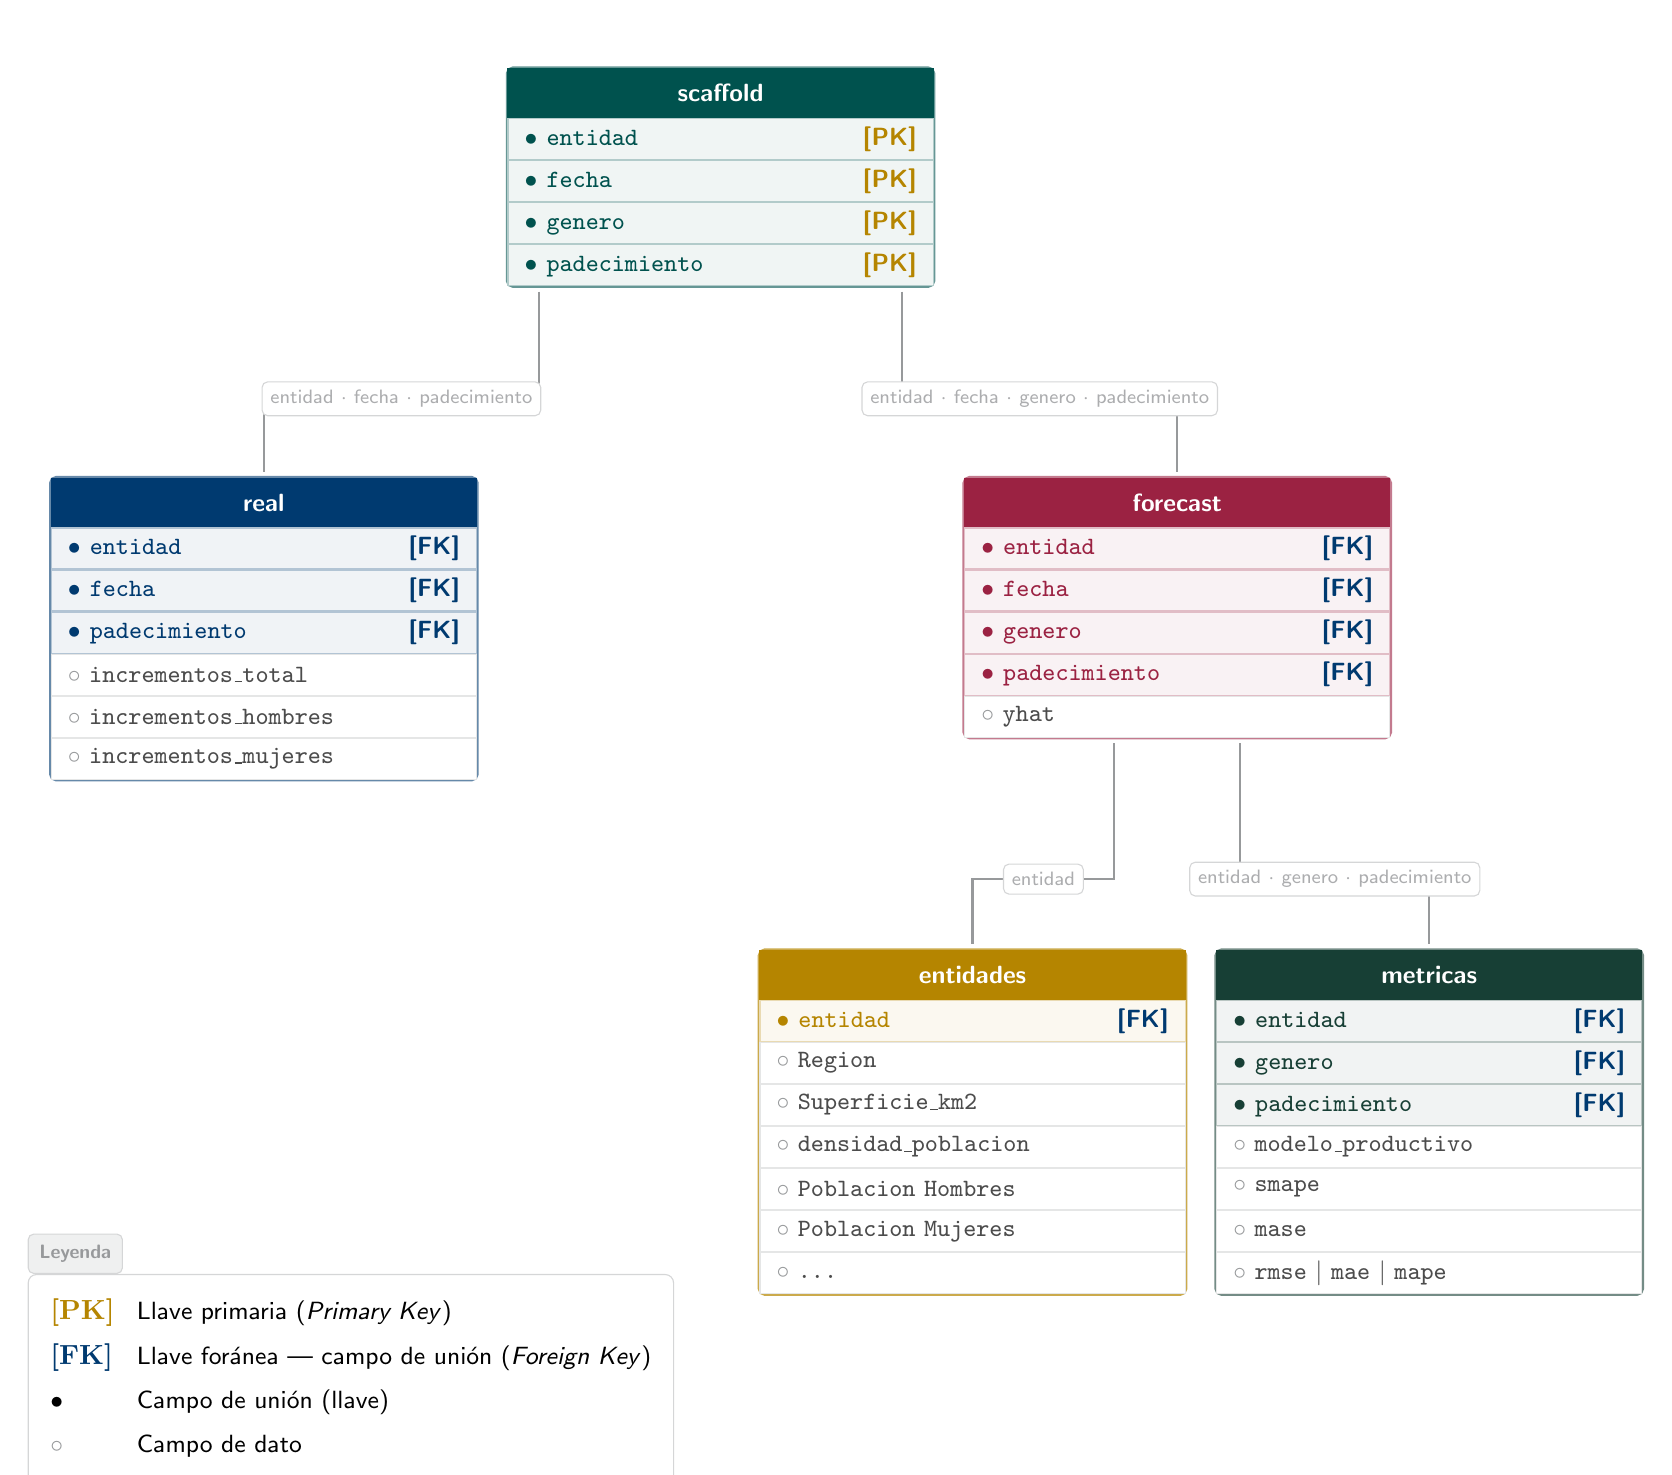
\begin{tikzpicture}[node distance=0pt]
% SCAFFOLD
\node[dbheader=teal] (sc_hdr) at (0,0) {scaffold};
\node[dbkeyrow=teal,  below=0pt of sc_hdr] (sc_r1) {\keyicon\texttt{entidad}\hfill\erdpk};
\node[dbkeyrow=teal,  below=0pt of sc_r1]  (sc_r2) {\keyicon\texttt{fecha}\hfill\erdpk};
\node[dbkeyrow=teal,  below=0pt of sc_r2]  (sc_r3) {\keyicon\texttt{genero}\hfill\erdpk};
\node[dbkeyrow=teal,  below=0pt of sc_r3]  (sc_r4) {\keyicon\texttt{padecimiento}\hfill\erdpk};
\begin{pgfonlayer}{background}
  \draw[draw=teal!60, line width=1.2pt, rounded corners=2pt]
    (sc_hdr.north west) rectangle (sc_r4.south east);
\end{pgfonlayer}
% REAL
\node[dbheader=imssblue] (rl_hdr) at (-5.8,-5.2) {real};
\node[dbkeyrow=imssblue,  below=0pt of rl_hdr] (rl_r1) {\keyicon\texttt{entidad}\hfill\erdfk};
\node[dbkeyrow=imssblue,  below=0pt of rl_r1]  (rl_r2) {\keyicon\texttt{fecha}\hfill\erdfk};
\node[dbkeyrow=imssblue,  below=0pt of rl_r2]  (rl_r3) {\keyicon\texttt{padecimiento}\hfill\erdfk};
\node[dbdatarow,           below=0pt of rl_r3]  (rl_r4) {\dataicon\texttt{incrementos\_total}};
\node[dbdatarow,           below=0pt of rl_r4]  (rl_r5) {\dataicon\texttt{incrementos\_hombres}};
\node[dbdatarow,           below=0pt of rl_r5]  (rl_r6) {\dataicon\texttt{incrementos\_mujeres}};
\begin{pgfonlayer}{background}
  \draw[draw=imssblue!60, line width=1.2pt, rounded corners=2pt]
    (rl_hdr.north west) rectangle (rl_r6.south east);
\end{pgfonlayer}
% FORECAST
\node[dbheader=burgundy] (fc_hdr) at (5.8,-5.2) {forecast};
\node[dbkeyrow=burgundy,  below=0pt of fc_hdr] (fc_r1) {\keyicon\texttt{entidad}\hfill\erdfk};
\node[dbkeyrow=burgundy,  below=0pt of fc_r1]  (fc_r2) {\keyicon\texttt{fecha}\hfill\erdfk};
\node[dbkeyrow=burgundy,  below=0pt of fc_r2]  (fc_r3) {\keyicon\texttt{genero}\hfill\erdfk};
\node[dbkeyrow=burgundy,  below=0pt of fc_r3]  (fc_r4) {\keyicon\texttt{padecimiento}\hfill\erdfk};
\node[dbdatarow,           below=0pt of fc_r4]  (fc_r5) {\dataicon\texttt{yhat}};
\begin{pgfonlayer}{background}
  \draw[draw=burgundy!60, line width=1.2pt, rounded corners=2pt]
    (fc_hdr.north west) rectangle (fc_r5.south east);
\end{pgfonlayer}
% ENTIDADES
\node[dbheader=gold] (en_hdr) at (3.2,-11.2) {entidades};
\node[dbkeyrow=gold,  below=0pt of en_hdr] (en_r1) {\keyicon\texttt{entidad}\hfill\erdfk};
\node[dbdatarow,       below=0pt of en_r1]  (en_r2) {\dataicon\texttt{Region}};
\node[dbdatarow,       below=0pt of en_r2]  (en_r3) {\dataicon\texttt{Superficie\_km2}};
\node[dbdatarow,       below=0pt of en_r3]  (en_r4) {\dataicon\texttt{densidad\_poblacion}};
\node[dbdatarow,       below=0pt of en_r4]  (en_r5) {\dataicon\texttt{Poblacion Hombres}};
\node[dbdatarow,       below=0pt of en_r5]  (en_r6) {\dataicon\texttt{Poblacion Mujeres}};
\node[dbdatarow,       below=0pt of en_r6]  (en_r7) {\dataicon\texttt{...}};
\begin{pgfonlayer}{background}
  \draw[draw=gold!70, line width=1.2pt, rounded corners=2pt]
    (en_hdr.north west) rectangle (en_r7.south east);
\end{pgfonlayer}
% METRICAS
\node[dbheader=darkteal] (mt_hdr) at (9.0,-11.2) {metricas};
\node[dbkeyrow=darkteal,  below=0pt of mt_hdr] (mt_r1) {\keyicon\texttt{entidad}\hfill\erdfk};
\node[dbkeyrow=darkteal,  below=0pt of mt_r1]  (mt_r2) {\keyicon\texttt{genero}\hfill\erdfk};
\node[dbkeyrow=darkteal,  below=0pt of mt_r2]  (mt_r3) {\keyicon\texttt{padecimiento}\hfill\erdfk};
\node[dbdatarow,           below=0pt of mt_r3]  (mt_r4) {\dataicon\texttt{modelo\_productivo}};
\node[dbdatarow,           below=0pt of mt_r4]  (mt_r5) {\dataicon\texttt{smape}};
\node[dbdatarow,           below=0pt of mt_r5]  (mt_r6) {\dataicon\texttt{mase}};
\node[dbdatarow,           below=0pt of mt_r6]  (mt_r7) {\dataicon\texttt{rmse\ $|$\ mae\ $|$\ mape}};
\begin{pgfonlayer}{background}
  \draw[draw=darkteal!60, line width=1.2pt, rounded corners=2pt]
    (mt_hdr.north west) rectangle (mt_r7.south east);
\end{pgfonlayer}
% CONNECTORS
\begin{pgfonlayer}{background}
\coordinate (sc_bl) at ($(sc_r4.south west)+(0.4,0)$);
\coordinate (rl_tc) at ($(rl_hdr.north)$);
\coordinate (elbow_rl) at ($(sc_bl |- rl_tc) + (0,1.0)$);
\draw[conn] (sc_bl) -- (sc_bl |- elbow_rl) -- (rl_tc |- elbow_rl) -- (rl_tc);
\node[joinlabel] at ($(sc_bl |- elbow_rl)!0.5!(rl_tc |- elbow_rl)$)
  {entidad $\cdot$ fecha $\cdot$ padecimiento};
\coordinate (sc_br) at ($(sc_r4.south east)+(-0.4,0)$);
\coordinate (fc_tc) at ($(fc_hdr.north)$);
\coordinate (elbow_fc) at ($(sc_br |- fc_tc) + (0,1.0)$);
\draw[conn] (sc_br) -- (sc_br |- elbow_fc) -- (fc_tc |- elbow_fc) -- (fc_tc);
\node[joinlabel] at ($(sc_br |- elbow_fc)!0.5!(fc_tc |- elbow_fc)$)
  {entidad $\cdot$ fecha $\cdot$ genero $\cdot$ padecimiento};
\coordinate (fc_bc) at ($(fc_r5.south)+(-0.8,0)$);
\coordinate (en_tc) at ($(en_hdr.north)$);
\coordinate (elbow_en) at ($(fc_bc |- en_tc) + (0,0.9)$);
\draw[conn] (fc_bc) -- (fc_bc |- elbow_en) -- (en_tc |- elbow_en) -- (en_tc);
\node[joinlabel] at ($(fc_bc |- elbow_en)!0.5!(en_tc |- elbow_en)$) {entidad};
\coordinate (fc_bc2) at ($(fc_r5.south)+(0.8,0)$);
\coordinate (mt_tc) at ($(mt_hdr.north)$);
\coordinate (elbow_mt) at ($(fc_bc2 |- mt_tc) + (0,0.9)$);
\draw[conn] (fc_bc2) -- (fc_bc2 |- elbow_mt) -- (mt_tc |- elbow_mt) -- (mt_tc);
\node[joinlabel] at ($(fc_bc2 |- elbow_mt)!0.5!(mt_tc |- elbow_mt)$)
  {entidad $\cdot$ genero $\cdot$ padecimiento};
\end{pgfonlayer}
% LEGEND
\node[rectangle, draw=coolgray!40, fill=white, rounded corners=3pt,
      inner sep=8pt, anchor=south west] (legend) at (-8.8, -18.0) {%
  \begin{tabular}{@{}l@{\hspace{8pt}}l@{}}
    \textcolor{gold}{\textbf{[PK]}}       & \sffamily\small Llave primaria (\textit{Primary Key}) \\[4pt]
    \textcolor{imssblue}{\textbf{[FK]}}   & \sffamily\small Llave foránea --- campo de unión (\textit{Foreign Key}) \\[4pt]
    {\small$\bullet$}                     & \sffamily\small Campo de unión (llave) \\[4pt]
    {\small\textcolor{coolgray}{$\circ$}} & \sffamily\small Campo de dato \\
  \end{tabular}};
\node[rectangle, fill=coolgray!15, draw=coolgray!40, rounded corners=2pt,
      inner sep=4pt, anchor=south west,
      font=\sffamily\bfseries\scriptsize\color{coolgray}]
      at (legend.north west) {Leyenda};
\end{tikzpicture}
}
\caption[Modelo entidad-relación del datasource de Tableau.]{%
Modelo entidad-relación de \texttt{tableau\_model.xlsx}: \texttt{scaffold}
como tabla ancla central, \texttt{real} y \texttt{forecast} en el segundo
nivel, y \texttt{entidades} y \texttt{metricas} como dimensiones colgadas
de \texttt{forecast}.}
\label{fig:erd}
\end{figure}

\subsection{Tabla \texttt{scaffold} como ancla central}

El diseño con \texttt{scaffold} como tabla ancla resuelve un problema crítico de Tableau: cuando los filtros se aplican sobre una tabla de hechos, no se propagan automáticamente a la otra tabla de hechos. Al colocar \texttt{scaffold} como nodo central y relacionar \texttt{real} y \texttt{forecast} a través de él, cualquier filtro aplicado sobre las dimensiones de \texttt{scaffold} (padecimiento, entidad, género) se propaga simultáneamente a ambas tablas de hechos. Esto garantiza que la serie histórica y el pronóstico respondan siempre al mismo filtro interactivo.

Adicionalmente, \texttt{scaffold} contiene la unión completa de fechas del histórico y del pronóstico, lo que permite que las visualizaciones muestren la serie continua sin interrupciones entre el último dato real y la primera predicción.

\begin{warningbox}[Filtros en Tableau: siempre desde \texttt{scaffold}]
Los filtros interactivos del dashboard (padecimiento, entidad, género, fecha) deben originarse siempre en los campos de \texttt{scaffold}, nunca en \texttt{real.*} ni en \texttt{forecast.*} directamente. De lo contrario, solo una de las dos tablas de hechos responderá al filtro.
\end{warningbox}

\subsection{Campo calculado \texttt{Calc\_Y\_Selected}}

La tabla \texttt{real} mantiene una sola fila por \texttt{(ds, entidad, padecimiento)}, con tres columnas de incrementos: \texttt{incrementos\_total}, \texttt{incrementos\_hombres} e \texttt{incrementos\_mujeres}. Para que las visualizaciones que muestran la serie histórica respondan al filtro de género, se utiliza el campo calculado \texttt{Calc\_Y\_Selected} en Tableau, que selecciona dinámicamente la columna correcta según el valor de \texttt{scaffold.genero}:

\begin{table}[H]
\centering
\caption{Lógica del campo calculado \texttt{Calc\_Y\_Selected}}
\label{tab:calc}
\small
\begin{tabular}{l l}
\toprule
\textbf{Valor de \texttt{scaffold.genero}} & \textbf{Campo seleccionado en \texttt{real}} \\
\midrule
\texttt{general} & \texttt{incrementos\_total} \\
\texttt{hombres} & \texttt{incrementos\_hombres} \\
\texttt{mujeres} & \texttt{incrementos\_mujeres} \\
\bottomrule
\end{tabular}
\end{table}

\newpage
% =============================================================================
% 6. ARQUITECTURA DEL WORKBOOK DE TABLEAU
% =============================================================================
\section{Arquitectura del Workbook de Tableau}\label{sec:workbook}

El workbook \texttt{viz\_epiforecastmx.twb} está compuesto por \textbf{20 hojas de visualización} organizadas en \textbf{4 dashboards principales}.

\subsection{Dashboards principales}

\begin{table}[H]
\centering
\caption{Dashboards principales del workbook}
\label{tab:dashboards}
\small
\begin{tabularx}{\textwidth}{>{\bfseries}l X}
\toprule
\textbf{Dashboard} & \textbf{Propósito} \\
\midrule
DashNacional   & Visualización de predicciones epidemiológicas y series históricas a nivel nacional, con filtros por padecimiento y género. \\
DashRegional   & Visualización de predicciones agregadas por las cuatro regiones de salud mental, con comparativa interregional. \\
DashDesempeño  & Análisis a nivel estatal con visualización de predicciones por entidad federativa y métricas de desempeño del modelo asignado. \\
DashKPIs       & Dashboard de monitoreo del sistema de modelado: 333 modelos en producción, cobertura, distribución de algoritmos y métricas promedio del sistema. \\
\bottomrule
\end{tabularx}
\end{table}

\subsection{Inventario de hojas de visualización}

Las 20 hojas del workbook se agrupan en cuatro categorías funcionales:

\begin{table}[H]
\centering
\caption{Hojas de exploración de datos}
\label{tab:hojas_exploracion}
\small
\begin{tabularx}{\textwidth}{>{\bfseries}l X}
\toprule
\textbf{Hoja} & \textbf{Función} \\
\midrule
Tabla de datos      & Vista tabular del dataset epidemiológico consolidado; funciona como herramienta de validación y exploración. \\
Mapa de México      & Representación geográfica coroplética de variables epidemiológicas y demográficas por entidad federativa. \\
México en categorías & Clasificación territorial de entidades según región, densidad poblacional, superficie y ratio hombres-mujeres. \\
Casos por año       & Evolución anual de la incidencia normalizada por 100,000 habitantes, con desagregación por padecimiento y género. \\
Casos por semana    & Evolución semanal de la incidencia; permite identificar picos, estacionalidad y cambios abruptos. \\
\bottomrule
\end{tabularx}
\end{table}

\begin{table}[H]
\centering
\caption{Hojas de visualización de predicciones}
\label{tab:hojas_predicciones}
\small
\begin{tabularx}{\textwidth}{>{\bfseries}l X}
\toprule
\textbf{Hoja} & \textbf{Función} \\
\midrule
Nacional            & Serie histórica completa y pronóstico a 52 semanas a nivel país. \\
Nacional52Semanas   & Vista concentrada en las últimas 52 semanas reales y las siguientes 52 proyectadas. \\
Regional            & Pronóstico agregado por las cuatro regiones de salud mental. \\
Regional52Semanas   & Vista regional enfocada en el horizonte temporal reciente. \\
Predicciones        & Pronósticos con bandas de confianza al 80\% (\texttt{yhat\_lower}, \texttt{yhat\_upper}). \\
Últimas 52 semanas  & Comportamiento reciente de la serie en zoom temporal. \\
\bottomrule
\end{tabularx}
\end{table}

\begin{table}[H]
\centering
\caption{Hojas de métricas y evaluación del modelo}
\label{tab:hojas_metricas}
\small
\begin{tabularx}{\textwidth}{>{\bfseries}l X}
\toprule
\textbf{Hoja} & \textbf{Función} \\
\midrule
Desempeño del modelo  & Evaluación del desempeño de modelos individuales por serie. \\
Metrics               & Métricas de error (\smape{}, \mase{}, \rmse{}, \mae{}, \mape{}) por modelo y serie. \\
MetricsNacional       & Métricas de error agregadas a nivel nacional. \\
MetricsRegional       & Métricas de error agregadas por región de salud mental. \\
Métricos promedio por padecimiento & Promedio de métricas de error por enfermedad. \\
\bottomrule
\end{tabularx}
\end{table}

\begin{table}[H]
\centering
\caption{Hojas de indicadores del sistema}
\label{tab:hojas_kpis}
\small
\begin{tabularx}{\textwidth}{>{\bfseries}l X}
\toprule
\textbf{Hoja} & \textbf{Función} \\
\midrule
KPIsGenerales               & Indicadores agregados: total de modelos, cobertura, métricas promedio. \\
Total de Modelos            & Conteo de los 333 modelos de producción activos. \\
Distribución de modelos usados & Frecuencia de uso de cada algoritmo (DeepAR, Prophet, Ensemble, Stacking). \\
BarChart                    & Visualización auxiliar de barras para la distribución de algoritmos. \\
\bottomrule
\end{tabularx}
\end{table}

\newpage
% =============================================================================
% 8. VISUALIZACIONES EN EL DASHBOARD WEB
% =============================================================================
\section{Visualizaciones en el Dashboard Web}\label{sec:visualizaciones_web}

Las siguientes imágenes corresponden a las visualizaciones finales desplegadas en el dashboard web del proyecto, accesible en \url{https://proyectointegrador.org/epidashboard}. Cada figura muestra una vista interactiva embebida directamente desde Tableau Public; el usuario puede explorar cualquiera de ellas en su versión completa haciendo clic en el enlace \textit{View on Tableau Public} que aparece en la parte inferior de cada visualización embebida. Desde Tableau Public también es posible descargar el workbook completo (\texttt{viz\_epiforecastmx.twb}) para su uso en Tableau Desktop.

% -------------------------------------------------------------------------
% Exploración — Tabla de datos
% -------------------------------------------------------------------------
La vista \textbf{Tabla de datos} expone el dataset epidemiológico consolidado en formato tabular. Cada fila representa una observación semanal para una combinación de entidad, padecimiento y género, con sus respectivos valores históricos, pronósticos y métricas del modelo asignado. Esta vista cumple dos funciones: (1) como herramienta de \textbf{validación} para el equipo técnico, que puede inspeccionar directamente los valores del dataset publicado en Google Sheets y detectar inconsistencias; y (2) como herramienta de \textbf{exportación} para usuarios avanzados que necesiten los datos en formato tabular para análisis externos. Los filtros disponibles incluyen \textbf{padecimiento}, \textbf{entidad}, \textbf{género} y \textbf{rango de fechas}. La tabla puede ordenarse por cualquier columna y exportarse desde Tableau Public como archivo \texttt{.csv}.

\begin{figure}[H]
\centering
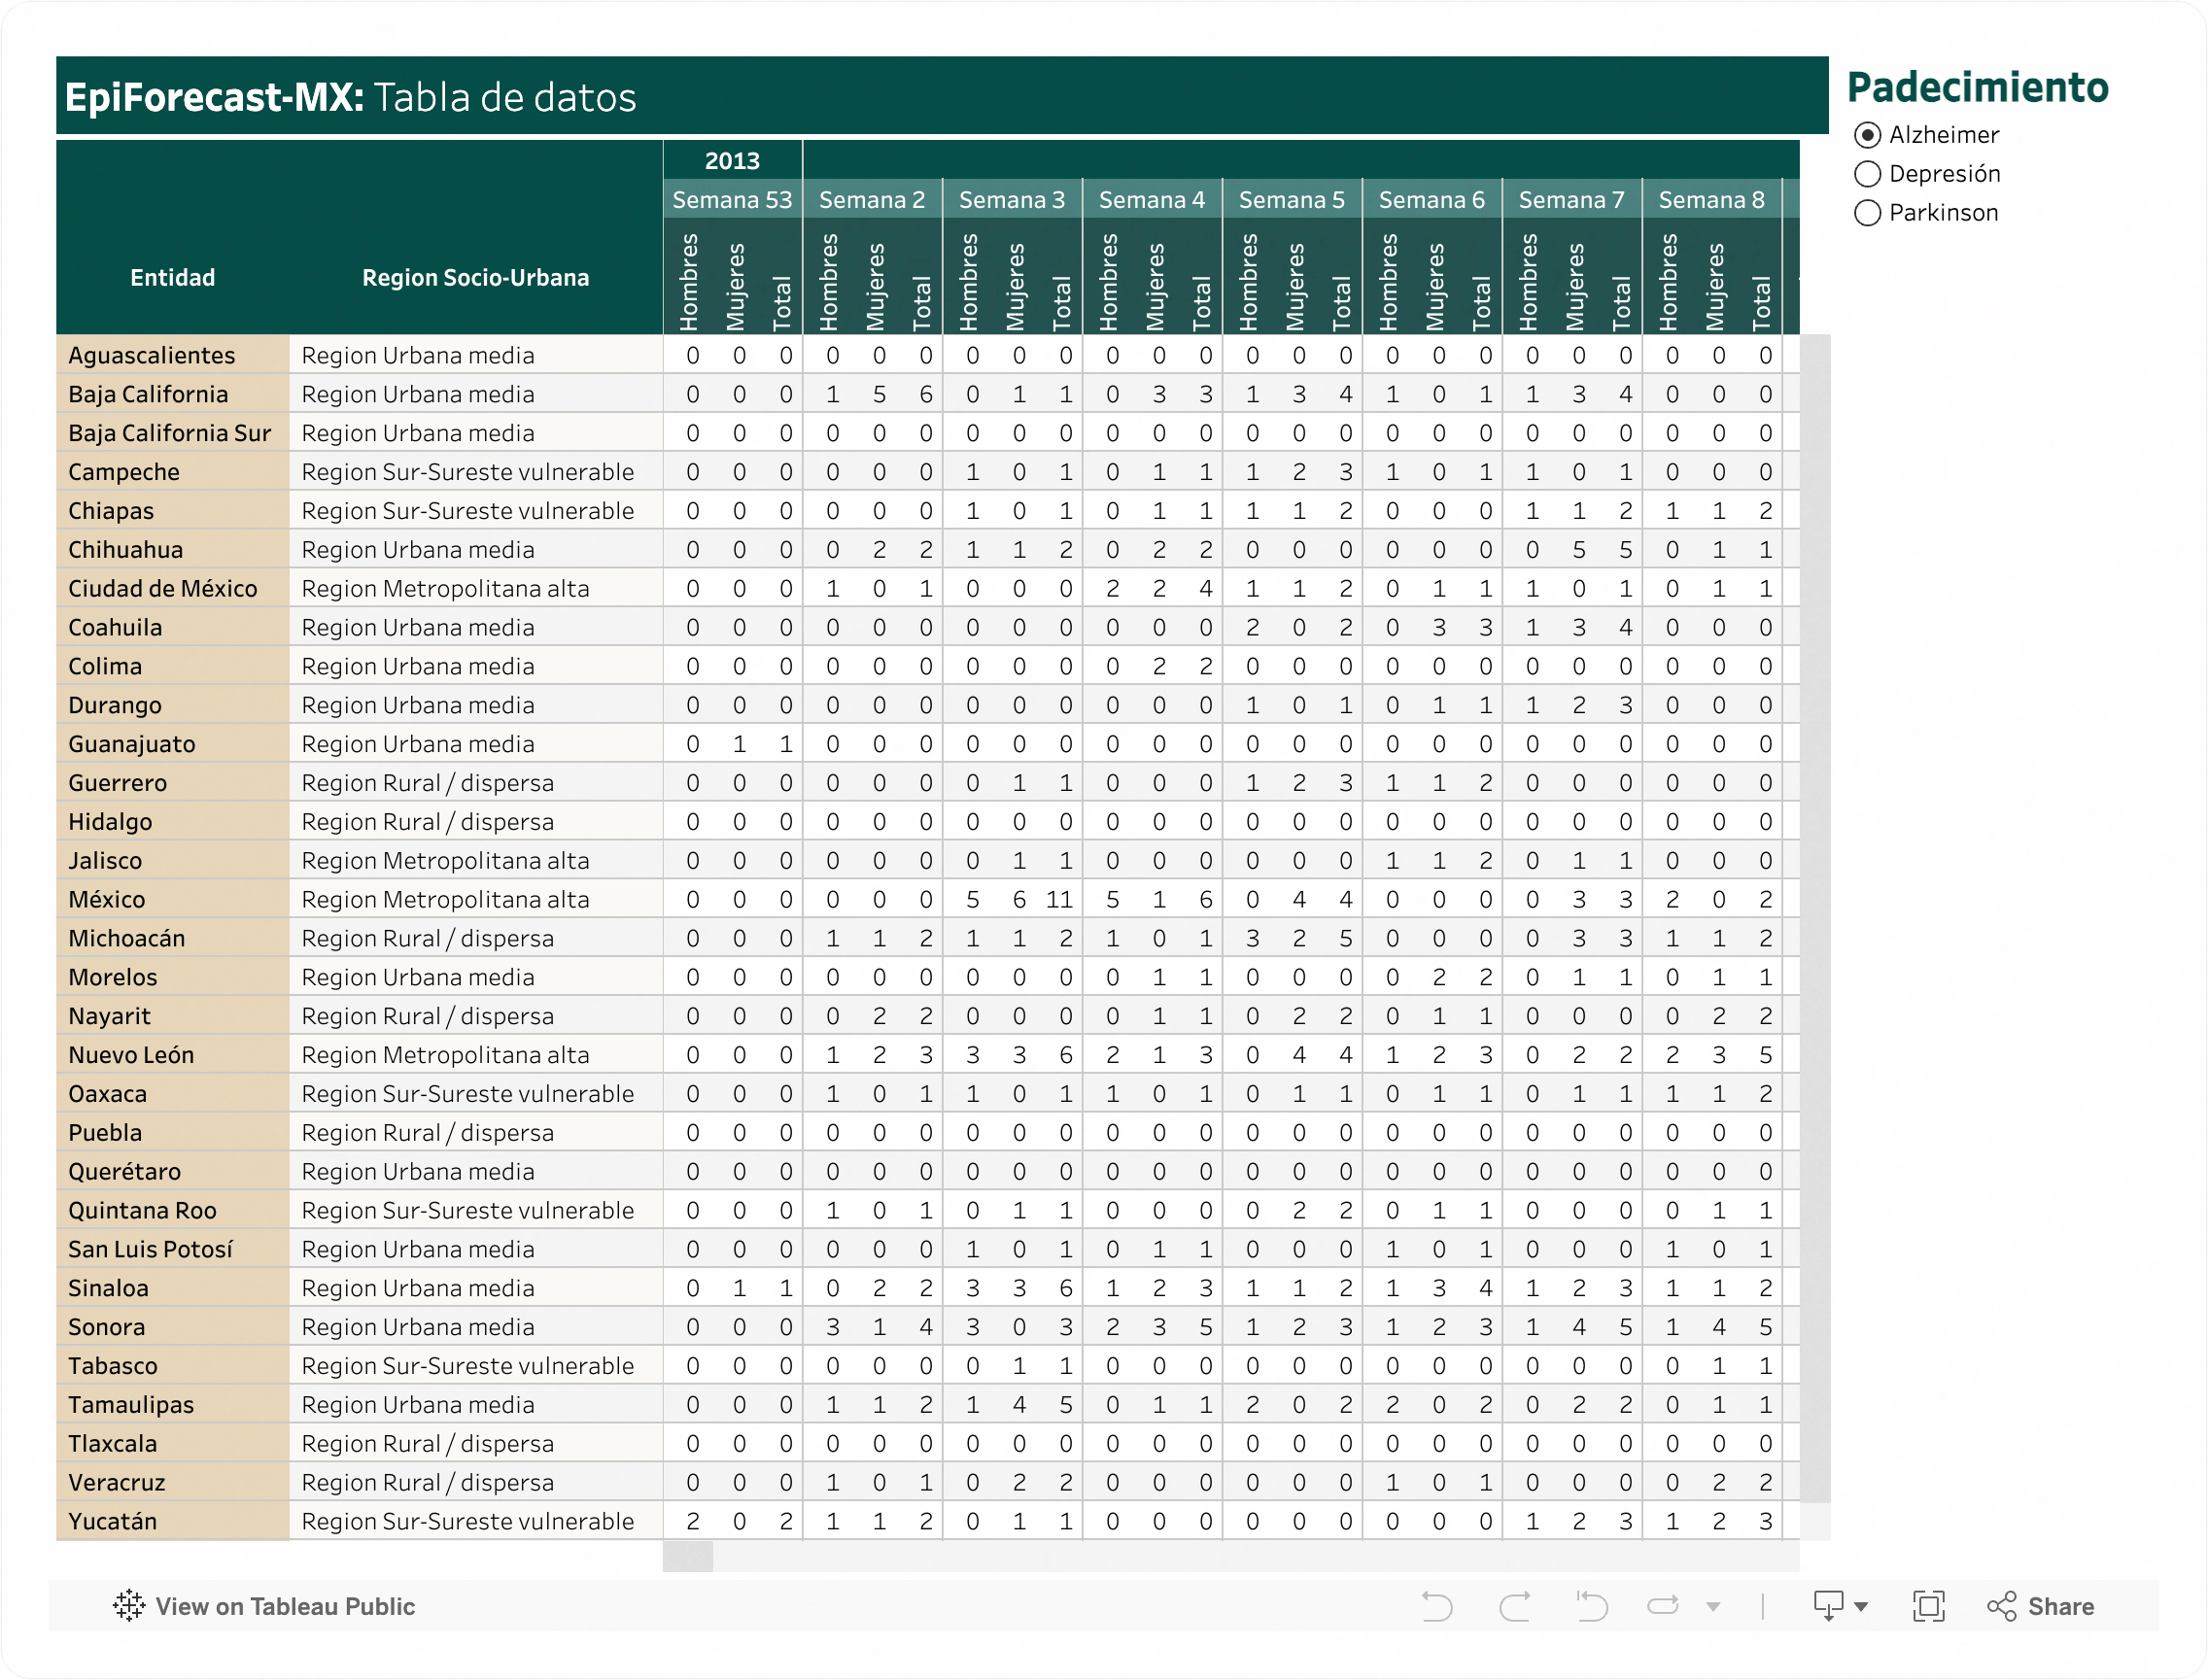
\includegraphics[width=0.80\textwidth]{FigurasTableau/explora-tabladedatos.png}
\caption[Exploración — Tabla de datos.]{Vista exploratoria \textbf{Tabla de datos}: acceso tabular al dataset epidemiológico consolidado; herramienta de validación y exploración detallada de registros.}
\label{fig:web_explora_tabla}
\end{figure}

\newpage
% -------------------------------------------------------------------------
% Exploración — Casos por año
% -------------------------------------------------------------------------
La vista \textbf{Casos por año} forma parte del módulo de exploración epidemiológica del dashboard. Muestra la evolución anual de la incidencia de casos, con desagregación por padecimiento y género. Permite identificar tendencias de largo plazo, el impacto del periodo COVID-19 (2020--2022) y la recuperación post-pandémica. El usuario puede filtrar por \textbf{padecimiento} (Depresión, Parkinson, Alzheimer), \textbf{género} (General, Hombres, Mujeres) y \textbf{entidad federativa}. Es especialmente útil para la planificación presupuestal anual y la comparación interanual de la carga de enfermedad.

\begin{figure}[H]
\centering
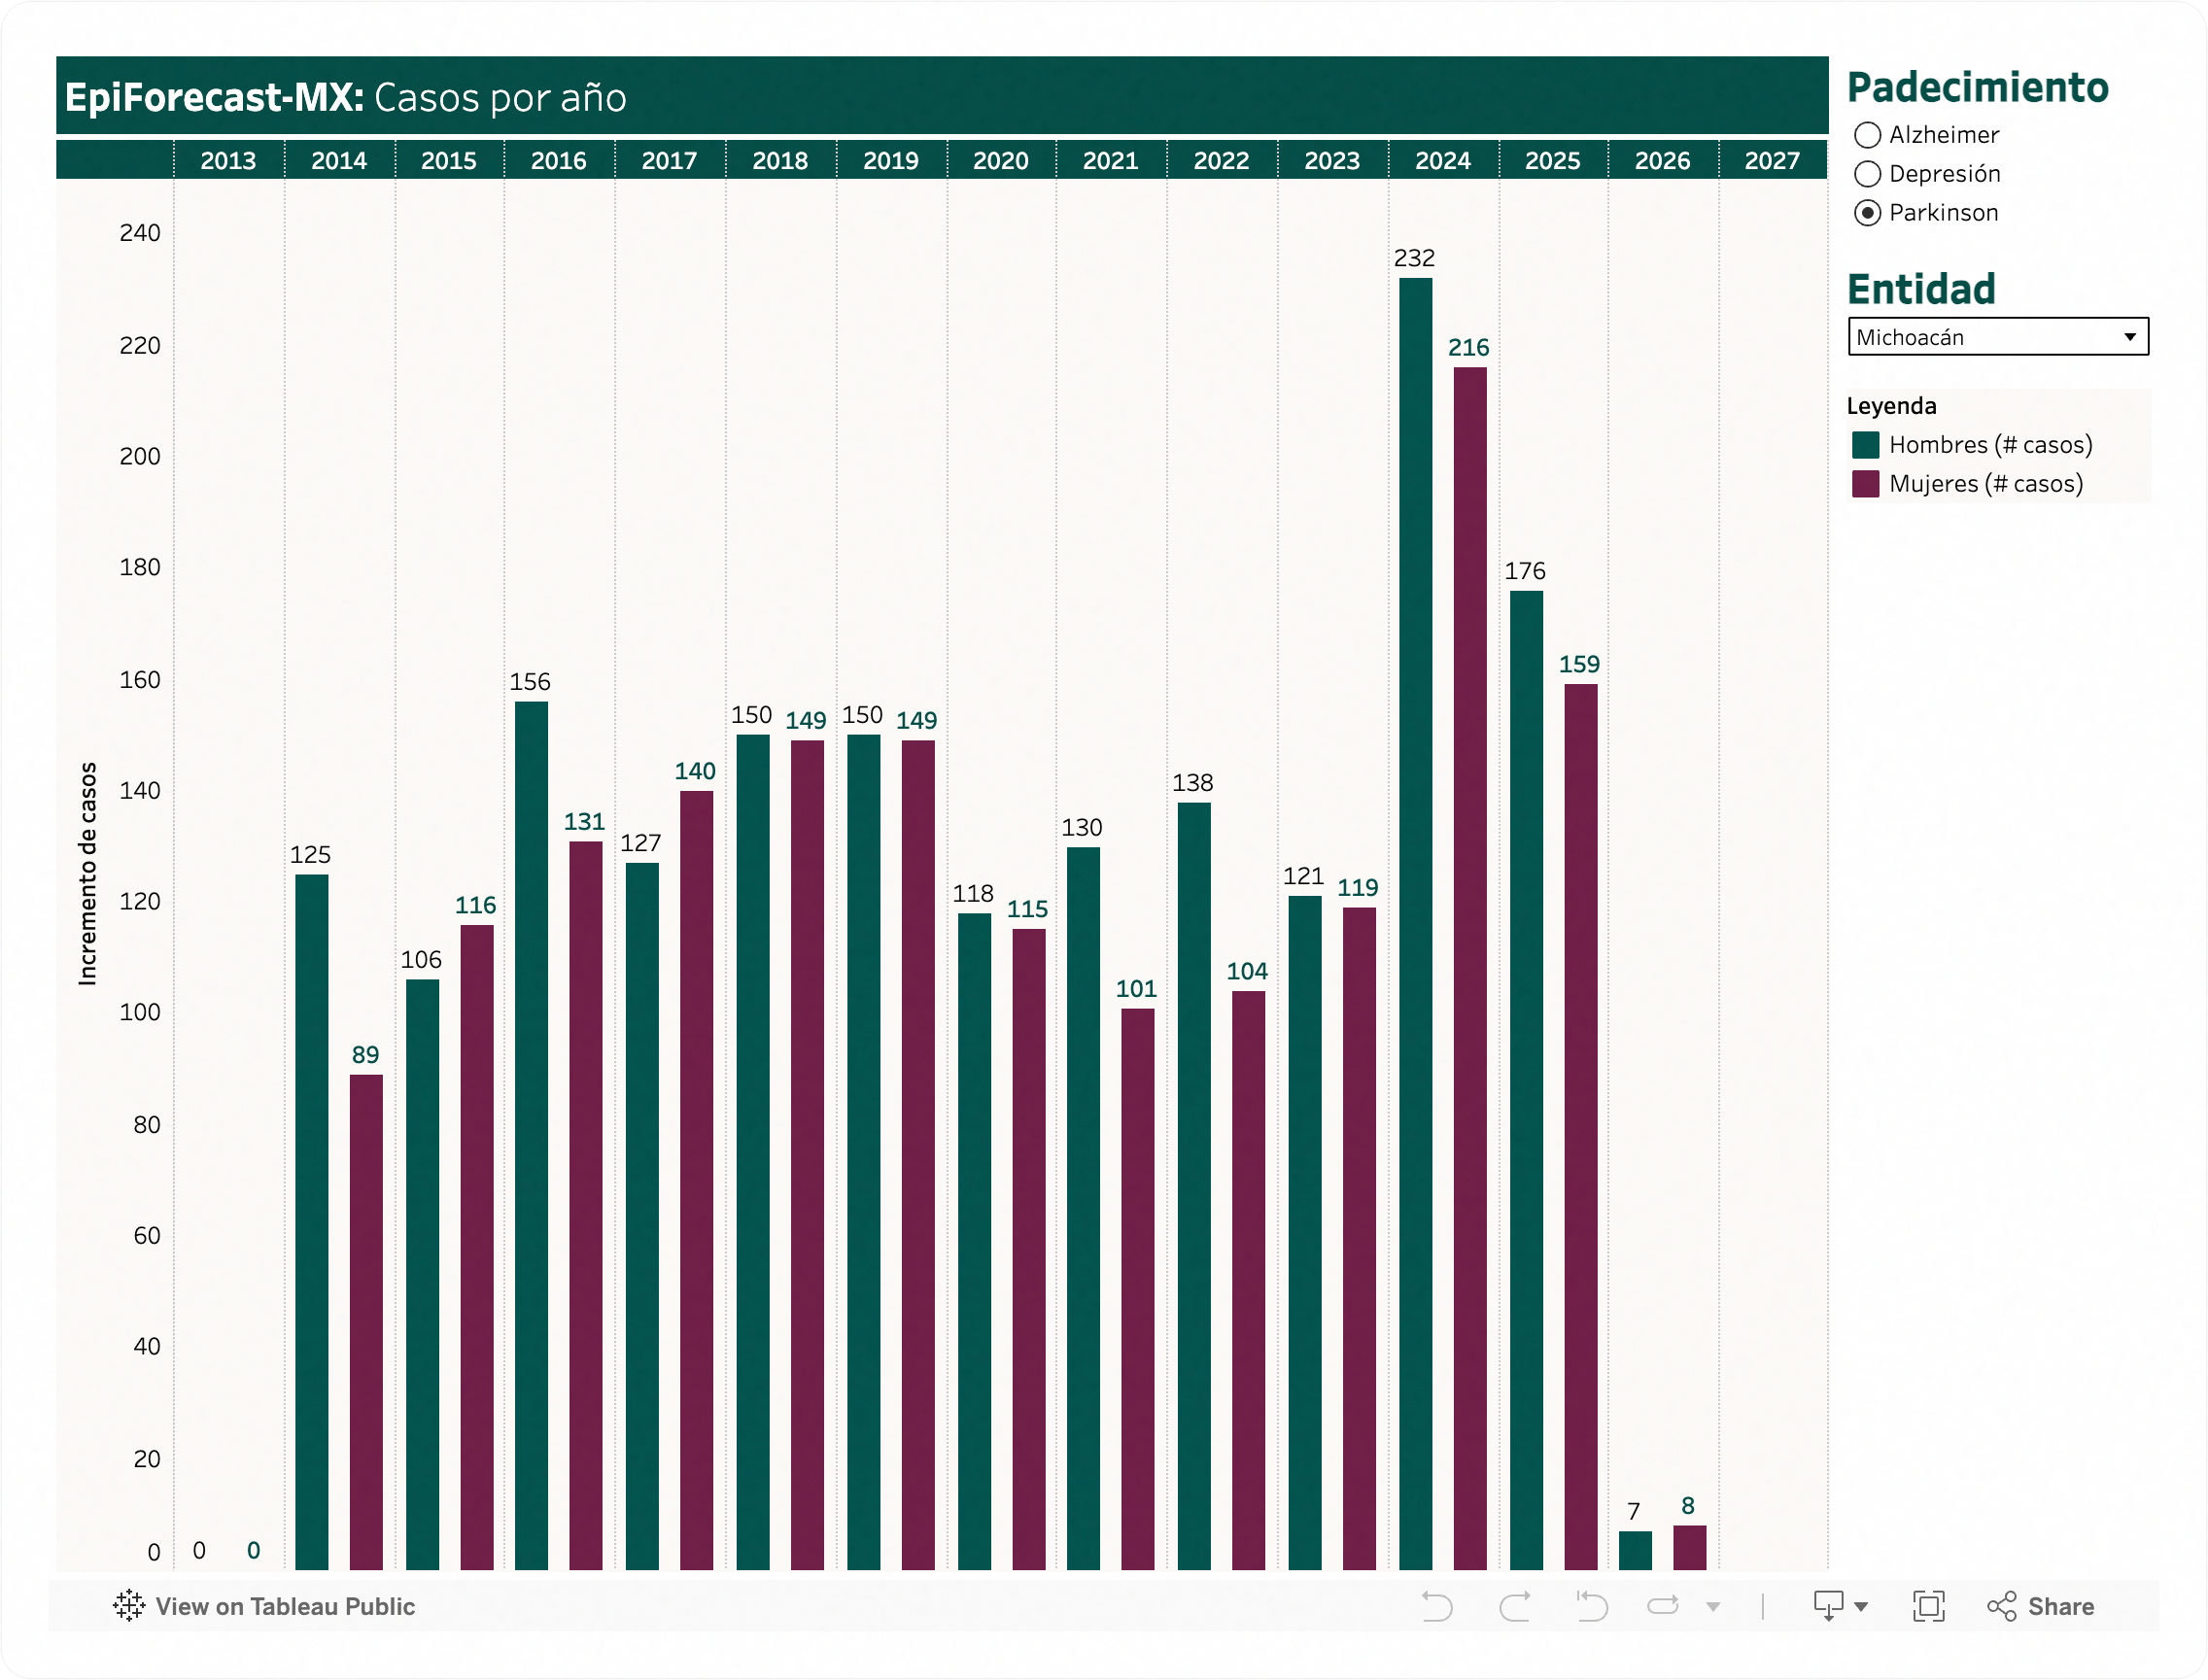
\includegraphics[width=\textwidth]{FigurasTableau/explora-casosporano.png}
\caption[Exploración — Casos por año.]{Vista exploratoria \textbf{Casos por año}: evolución anual de la incidencia normalizada por 100,000 habitantes, con desagregación por padecimiento y género.}
\label{fig:web_explora_casosporano}
\end{figure}

\newpage
% -------------------------------------------------------------------------
% Exploración — Casos por semana
% -------------------------------------------------------------------------
La vista \textbf{Casos por semana} presenta la evolución semanal de la incidencia a lo largo de todo el histórico disponible (2014--2026). A diferencia de la vista anual, esta resolución temporal permite identificar patrones finos: picos estacionales (como el incremento de Depresión en octubre y noviembre), cambios abruptos asociados a eventos exógenos (el desplome de consultas en 2020 durante el confinamiento por COVID-19) y la estacionalidad suave de Parkinson. Los filtros disponibles son \textbf{padecimiento}, \textbf{género} y \textbf{entidad federativa}. Esta vista es la herramienta principal para el epidemiólogo delegacional que necesita detectar semanas atípicas o validar que el comportamiento reciente de su estado es consistente con el patrón histórico.

\begin{figure}[H]
\centering
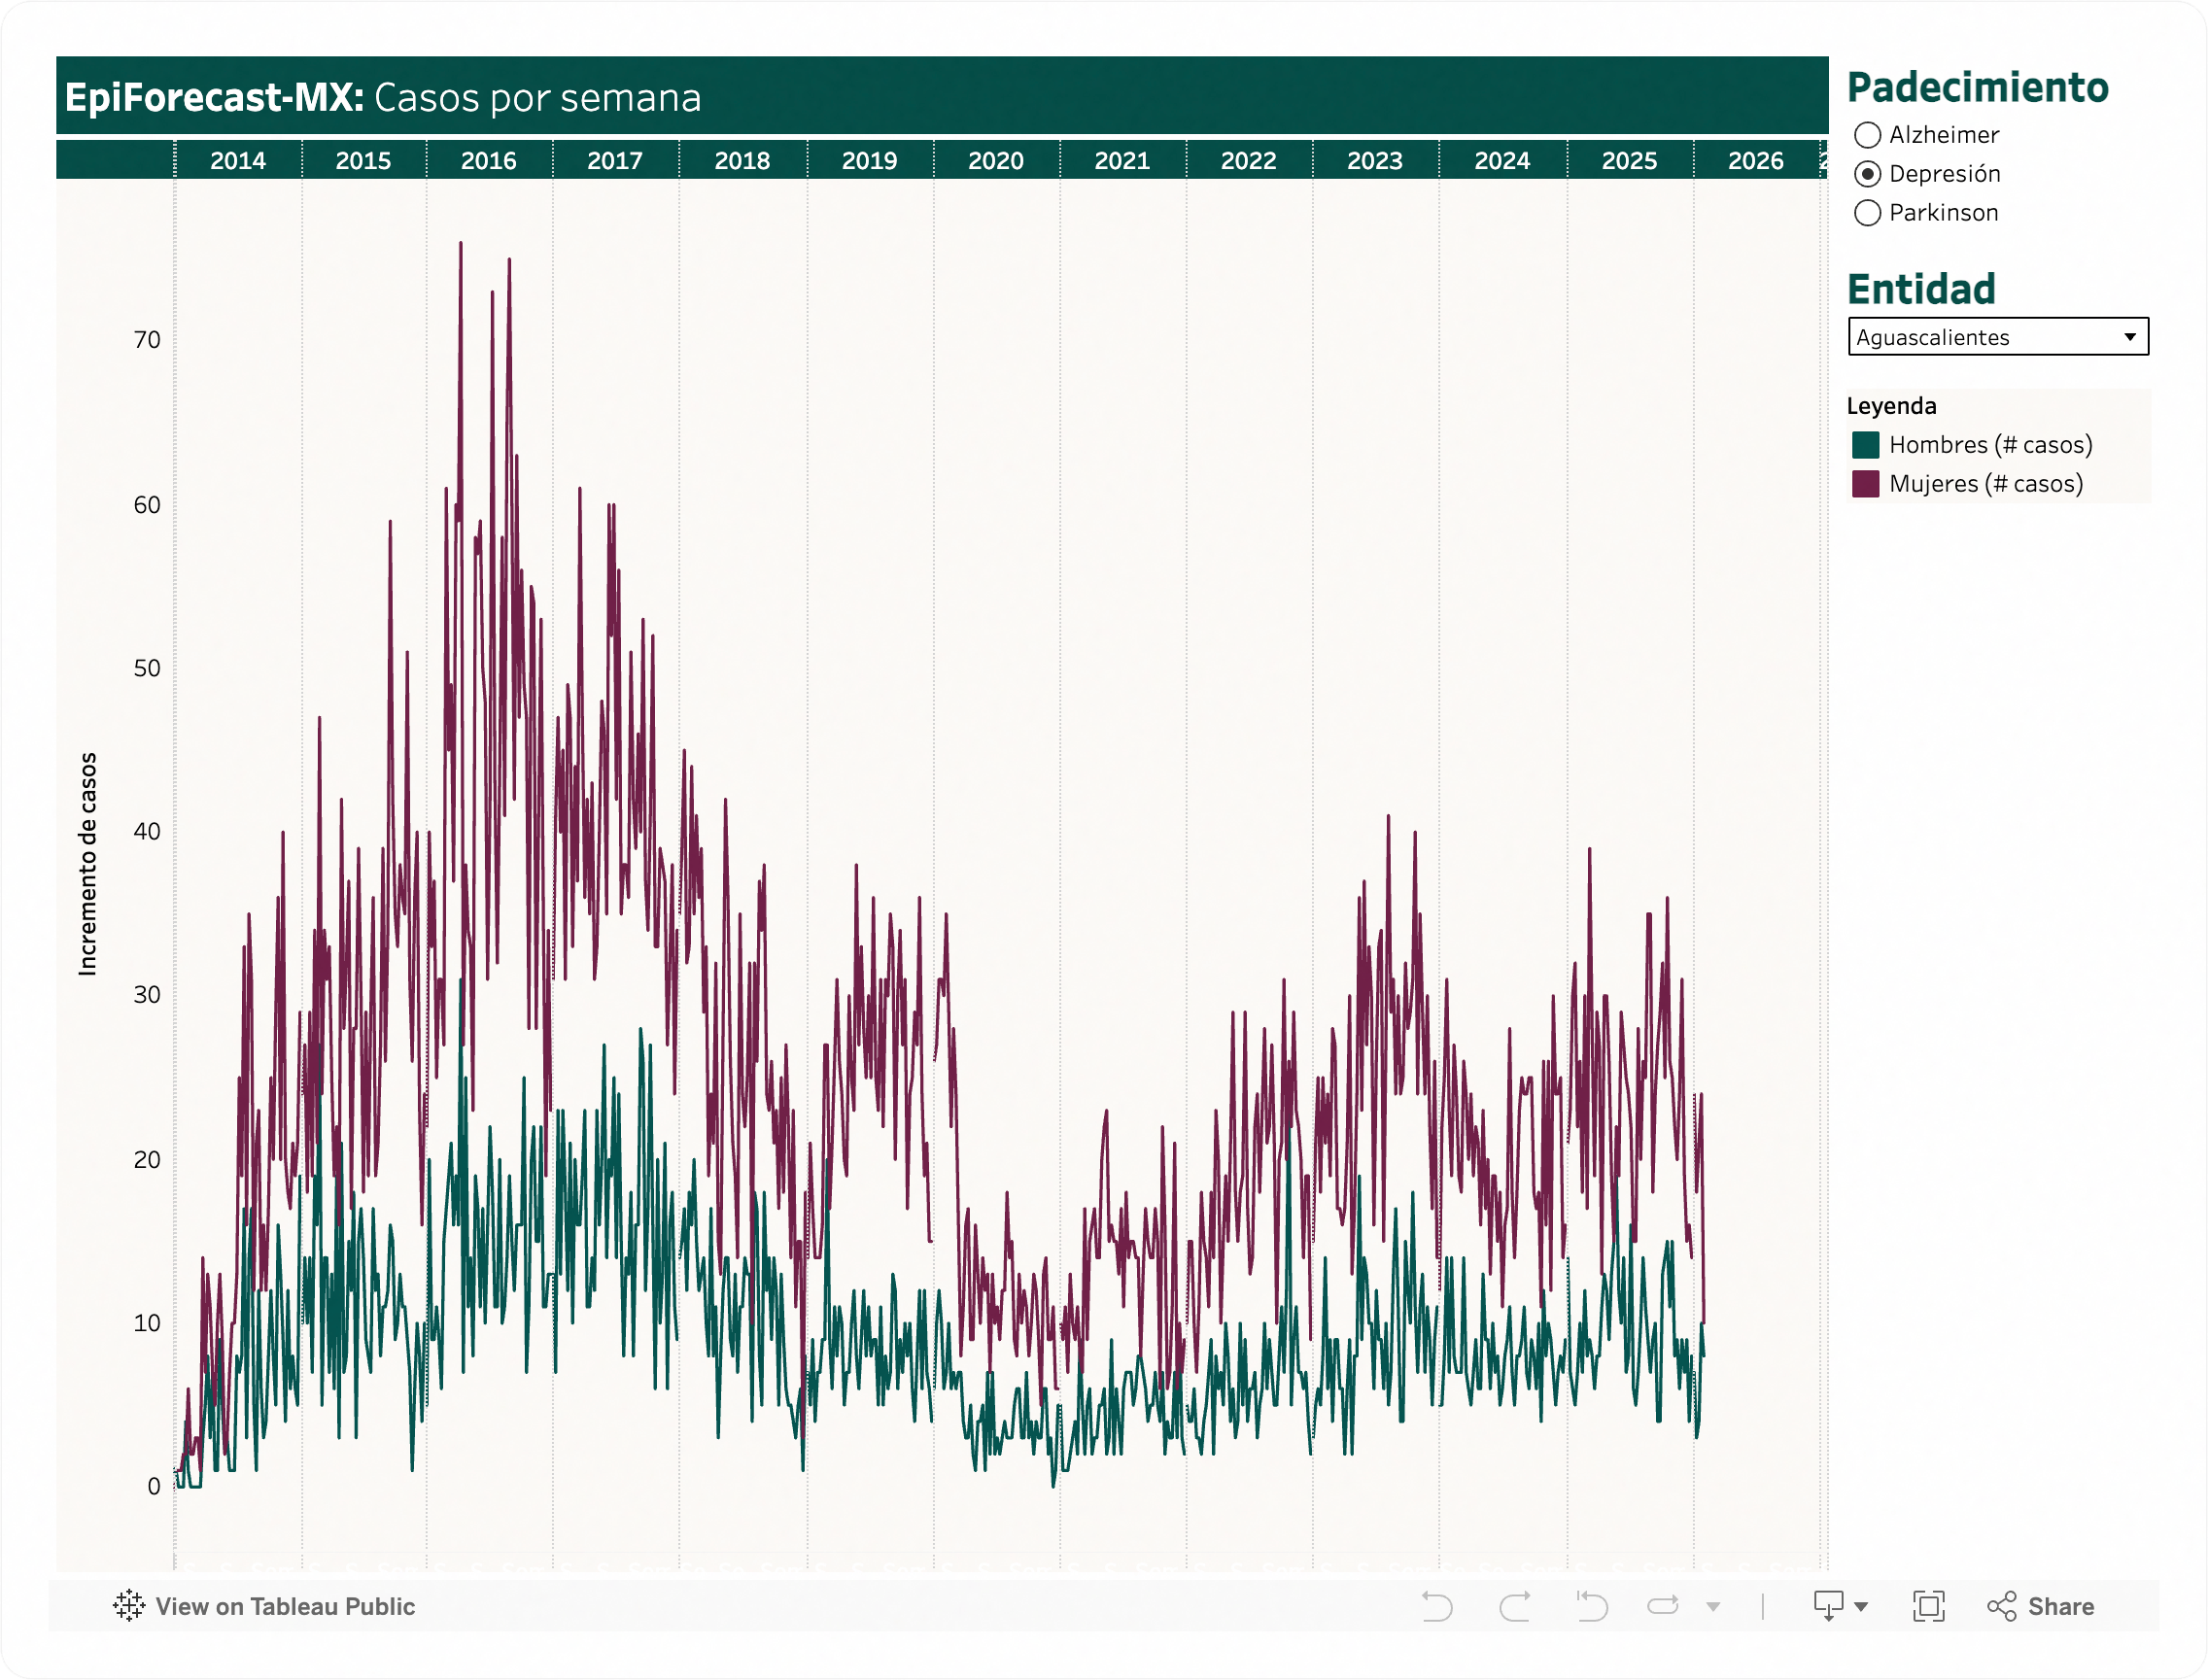
\includegraphics[width=\textwidth]{FigurasTableau/explora-casosporsemana.png}
\caption[Exploración — Casos por semana.]{Vista exploratoria \textbf{Casos por semana}: evolución semanal de la incidencia, útil para identificar picos, estacionalidad y cambios abruptos como el impacto de COVID-19.}
\label{fig:web_explora_casosporsemana}
\end{figure}

\newpage
% -------------------------------------------------------------------------
% Exploración — Mapa de México
% -------------------------------------------------------------------------
La vista \textbf{Mapa de México} ofrece una representación geográfica coroplética de la incidencia epidemiológica y variables demográficas del \textsc{inegi} por entidad federativa. La intensidad del color en cada estado codifica la variable seleccionada, permitiendo identificar de forma inmediata los estados con mayor carga de enfermedad y los patrones de distribución territorial. El usuario puede cambiar la variable desplegada en el mapa mediante el filtro de \textbf{métrica} (incidencia total, superficie, densidad poblacional, entre otras), así como filtrar por \textbf{padecimiento}. Al hacer clic sobre cualquier entidad, el mapa actúa como filtro de contexto que actualiza automáticamente las demás vistas del dashboard. Esta visualización es especialmente útil para comunicar la distribución espacial de la carga epidemiológica a directivos y tomadores de decisiones de nivel central.

\begin{figure}[H]
\centering
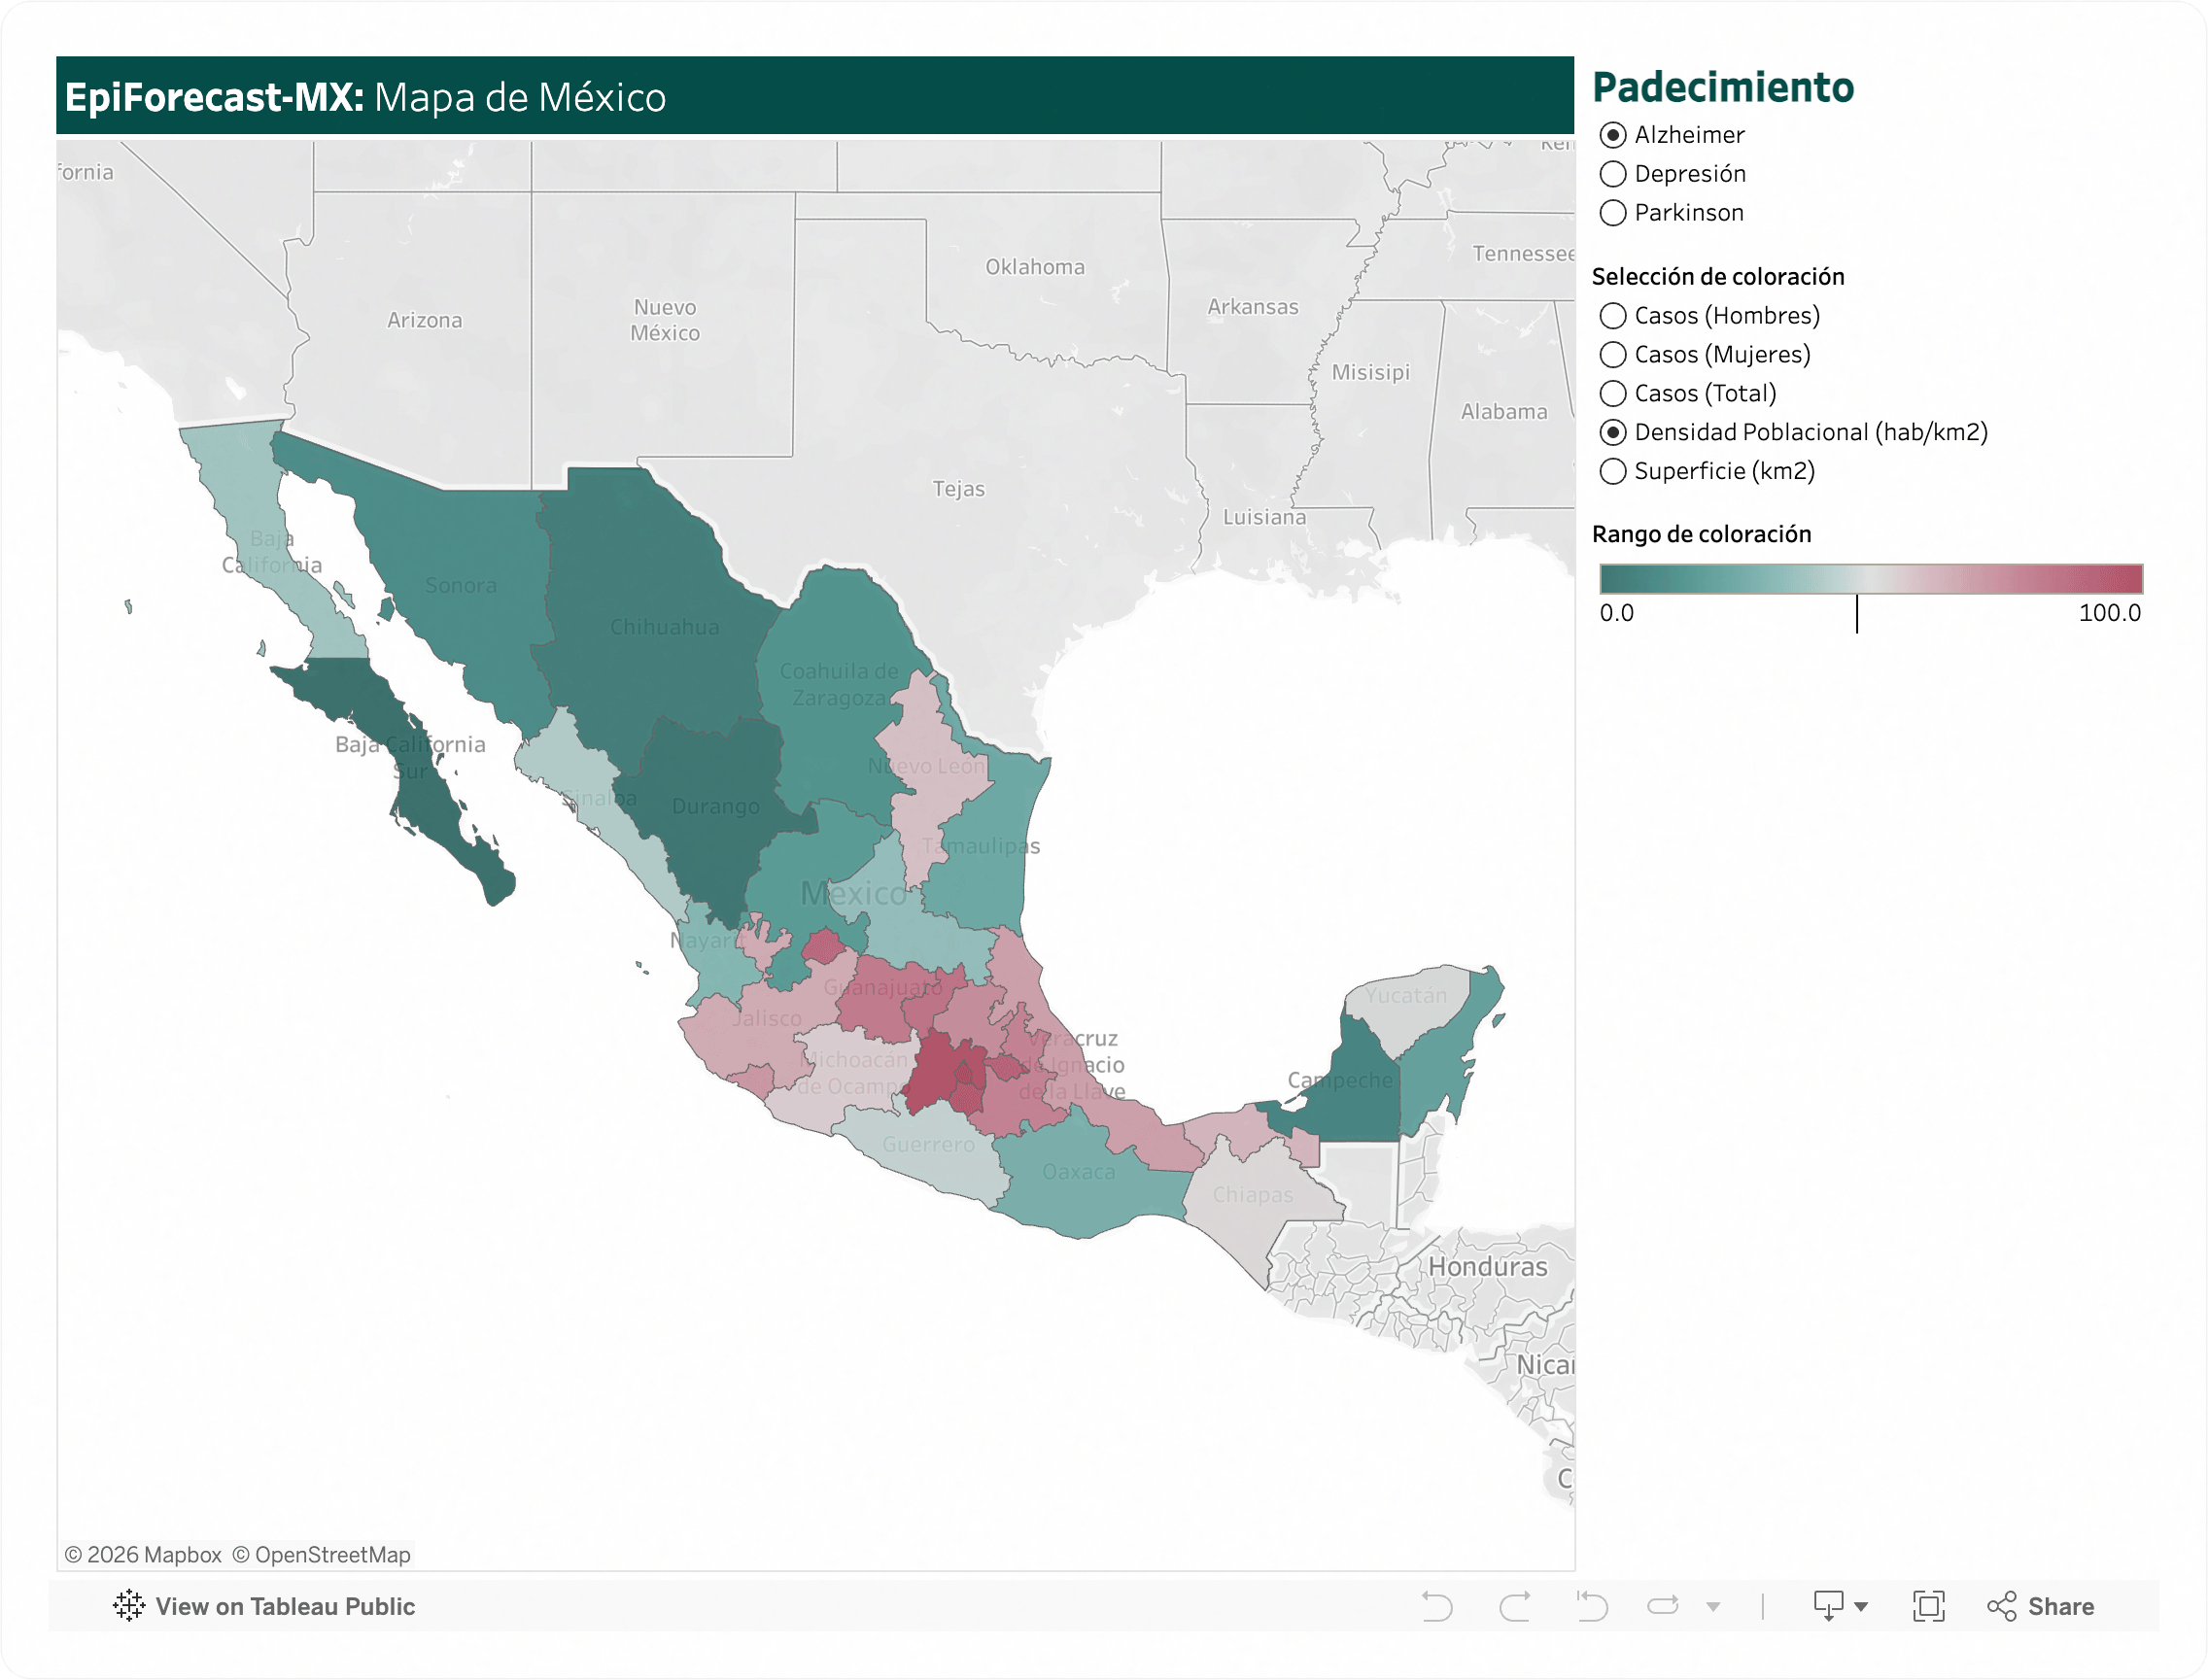
\includegraphics[width=\textwidth]{FigurasTableau/explora-mapademexico.png}
\caption[Exploración — Mapa de México.]{Vista exploratoria \textbf{Mapa de México}: representación geográfica coroplética de variables epidemiológicas y demográficas por entidad federativa.}
\label{fig:web_explora_mapa}
\end{figure}

\newpage
% -------------------------------------------------------------------------
% Exploración — México en categorías
% -------------------------------------------------------------------------
La vista \textbf{México en categorías} clasifica las 32 entidades federativas según atributos territoriales y socioeconómicos derivados del \textsc{inegi} (2024): región socioeconómica (Metropolitana alta, Urbana media, Rural/dispersa, Sur-Sureste vulnerable), densidad poblacional, superficie en km$^2$ y ratio hombres-mujeres. Esta segmentación ayuda a interpretar por qué ciertos estados obtienen mejores métricas de pronóstico que otros: los estados con mayor densidad y volumen de consultas tienden a producir series más estables y, por tanto, modelos más precisos. El usuario puede ordenar y filtrar las entidades por cualquiera de estas categorías. Esta vista no tiene un propósito de pronóstico directo, sino que provee el contexto demográfico y territorial necesario para interpretar correctamente las diferencias de rendimiento entre series.

\begin{figure}[H]
\centering
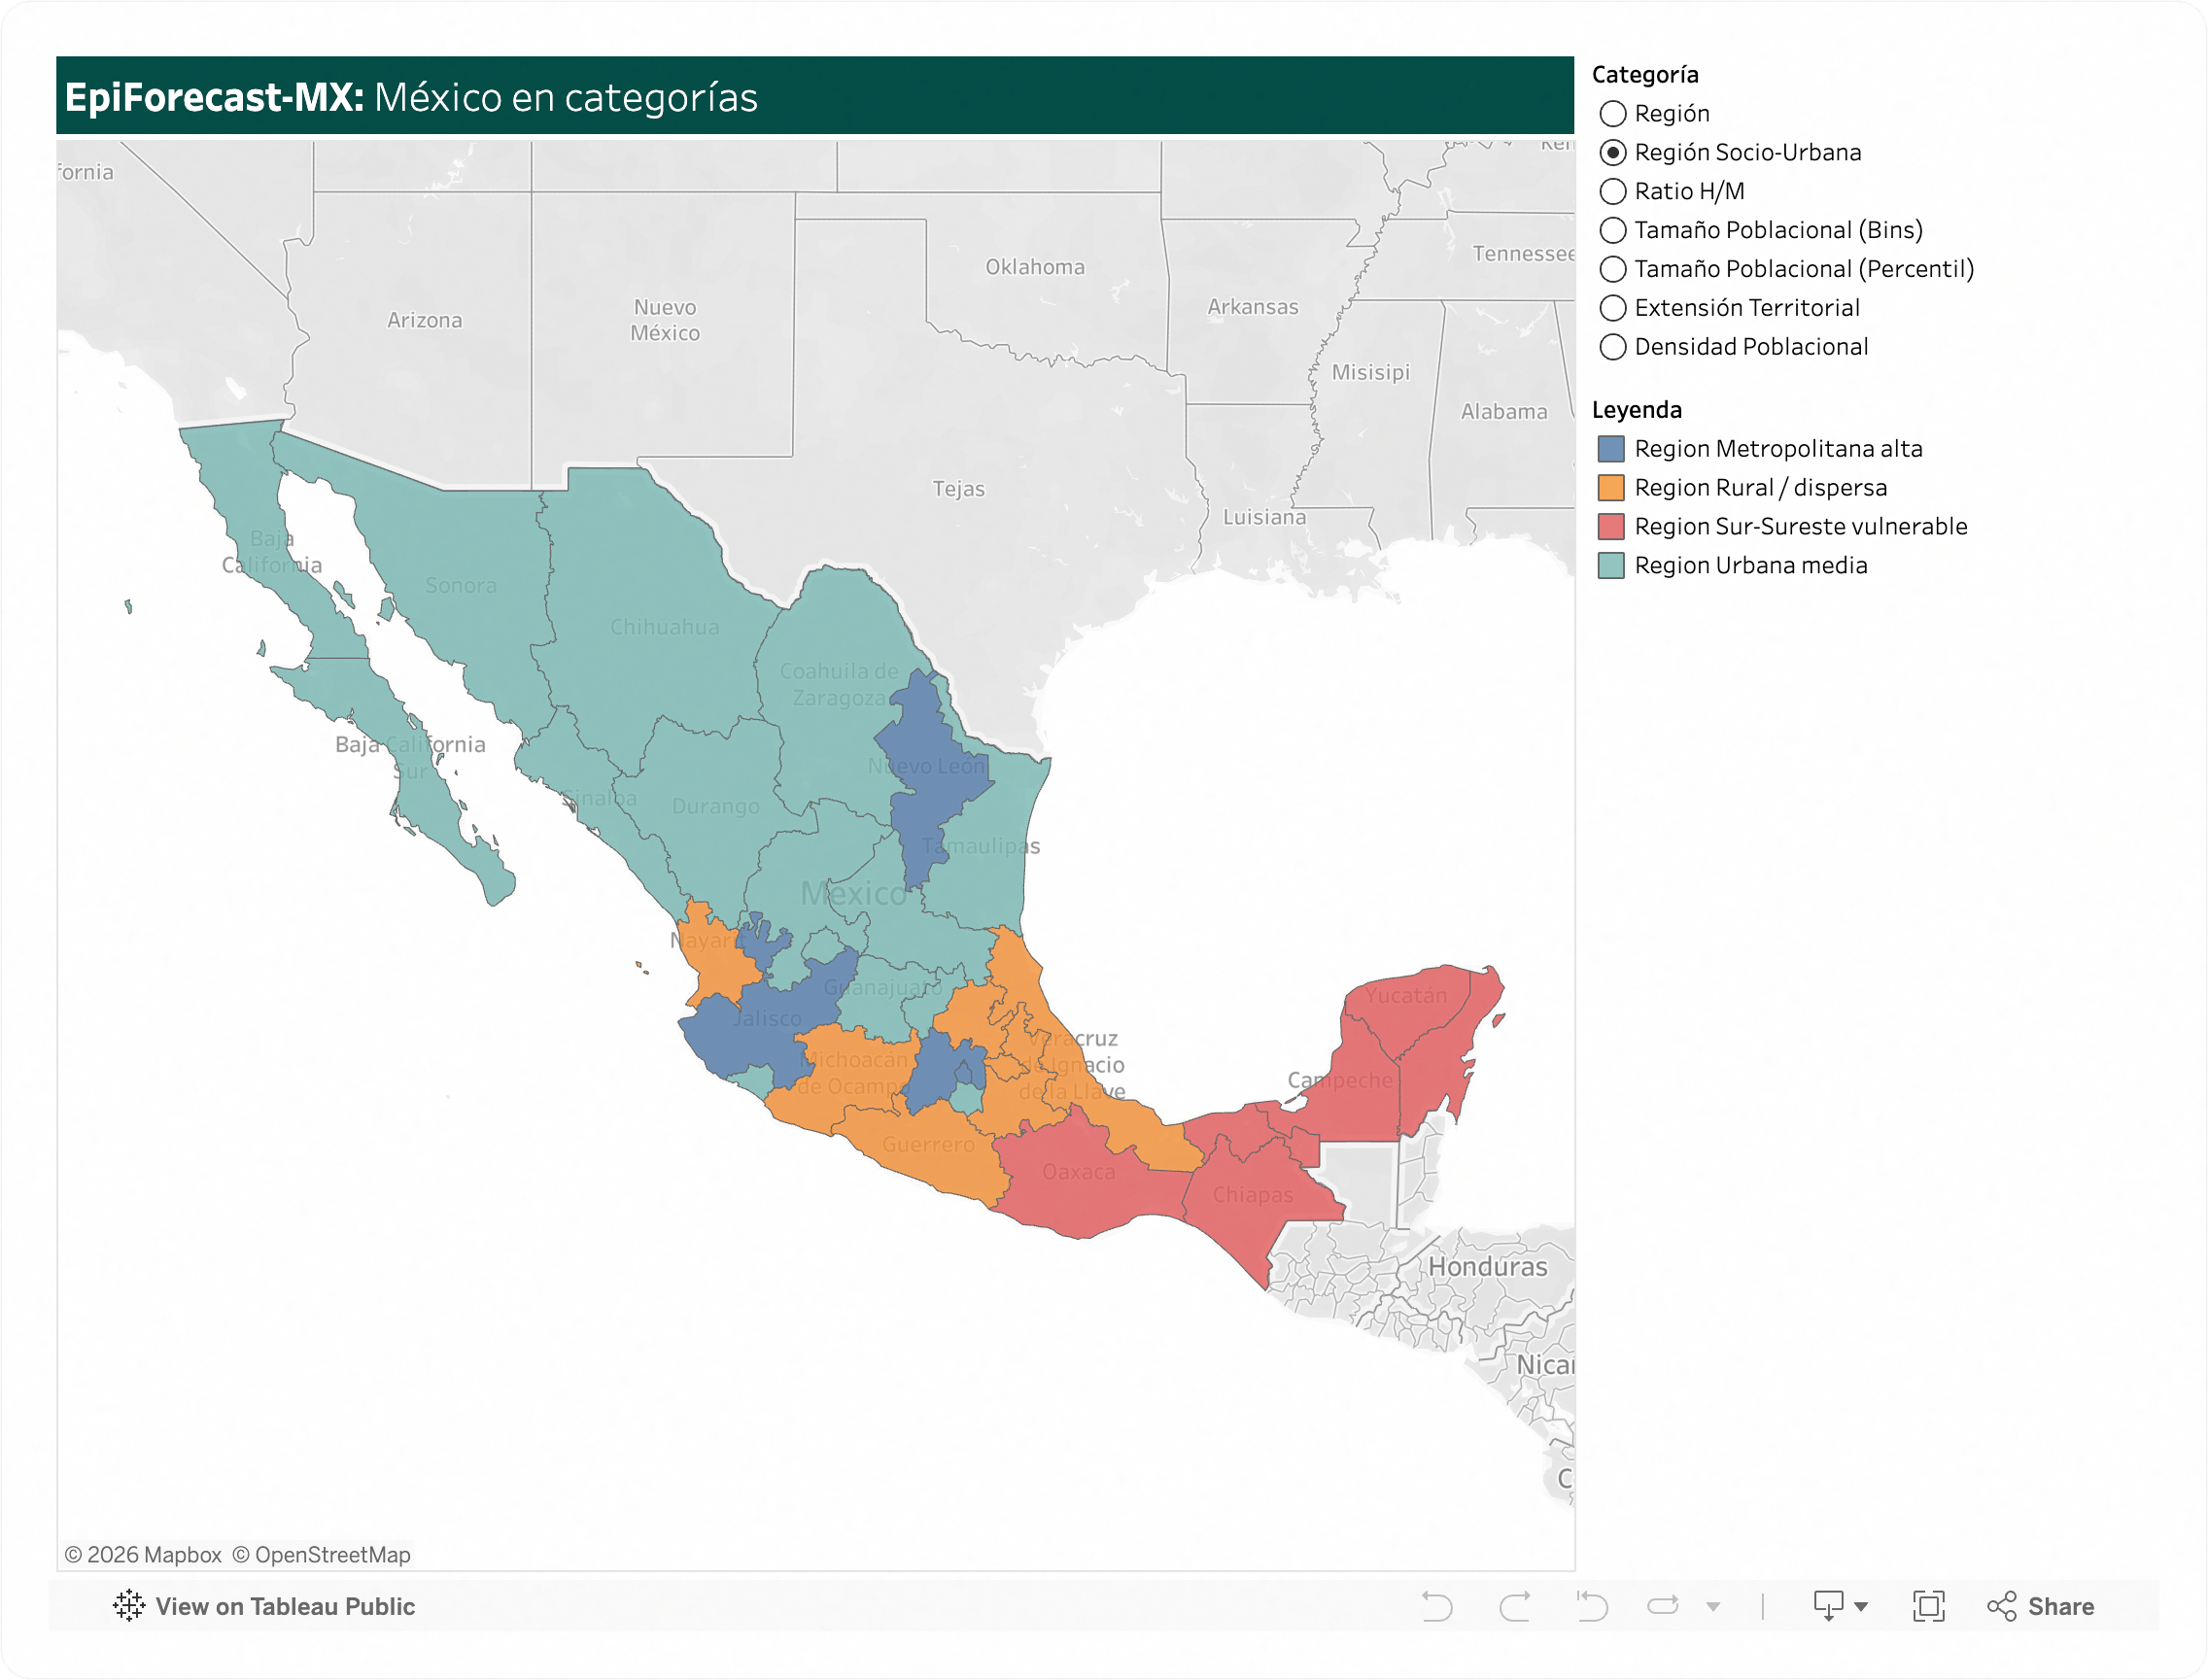
\includegraphics[width=\textwidth]{FigurasTableau/explora-mexicoencategorias.png}
\caption[Exploración — México en categorías.]{Vista exploratoria \textbf{México en categorías}: clasificación territorial de las 32 entidades según región socioeconómica, densidad poblacional, superficie y ratio hombres-mujeres.}
\label{fig:web_explora_categorias}
\end{figure}

\newpage

% -------------------------------------------------------------------------
% Predicción estatal con banda de confianza
% -------------------------------------------------------------------------
La vista \textbf{Predicción estatal con intervalo de confianza} corresponde a la hoja \textit{Predicciones} del workbook y es la visualización de mayor valor analítico para el epidemiólogo delegacional. Muestra el pronóstico a 52 semanas del modelo productivo asignado a la serie seleccionada, junto con las bandas de confianza al 80\% (\texttt{yhat\_lower} / \texttt{yhat\_upper}). Una banda estrecha refleja alta certeza del modelo (típica en series de Depresión con alto volumen); una banda ancha indica mayor incertidumbre (común en Alzheimer o Parkinson en estados pequeños). Los filtros disponibles son \textbf{padecimiento}, \textbf{entidad federativa} (incluyendo las 4 regiones y el nivel Nacional) y \textbf{género}. El panel lateral muestra el \smape{} del modelo activo y su calificación cualitativa. Esta vista es la herramienta recomendada para la toma de decisiones sobre aprovisionamiento de medicamentos e insumos con horizonte trimestral.

\begin{figure}[H]
\centering
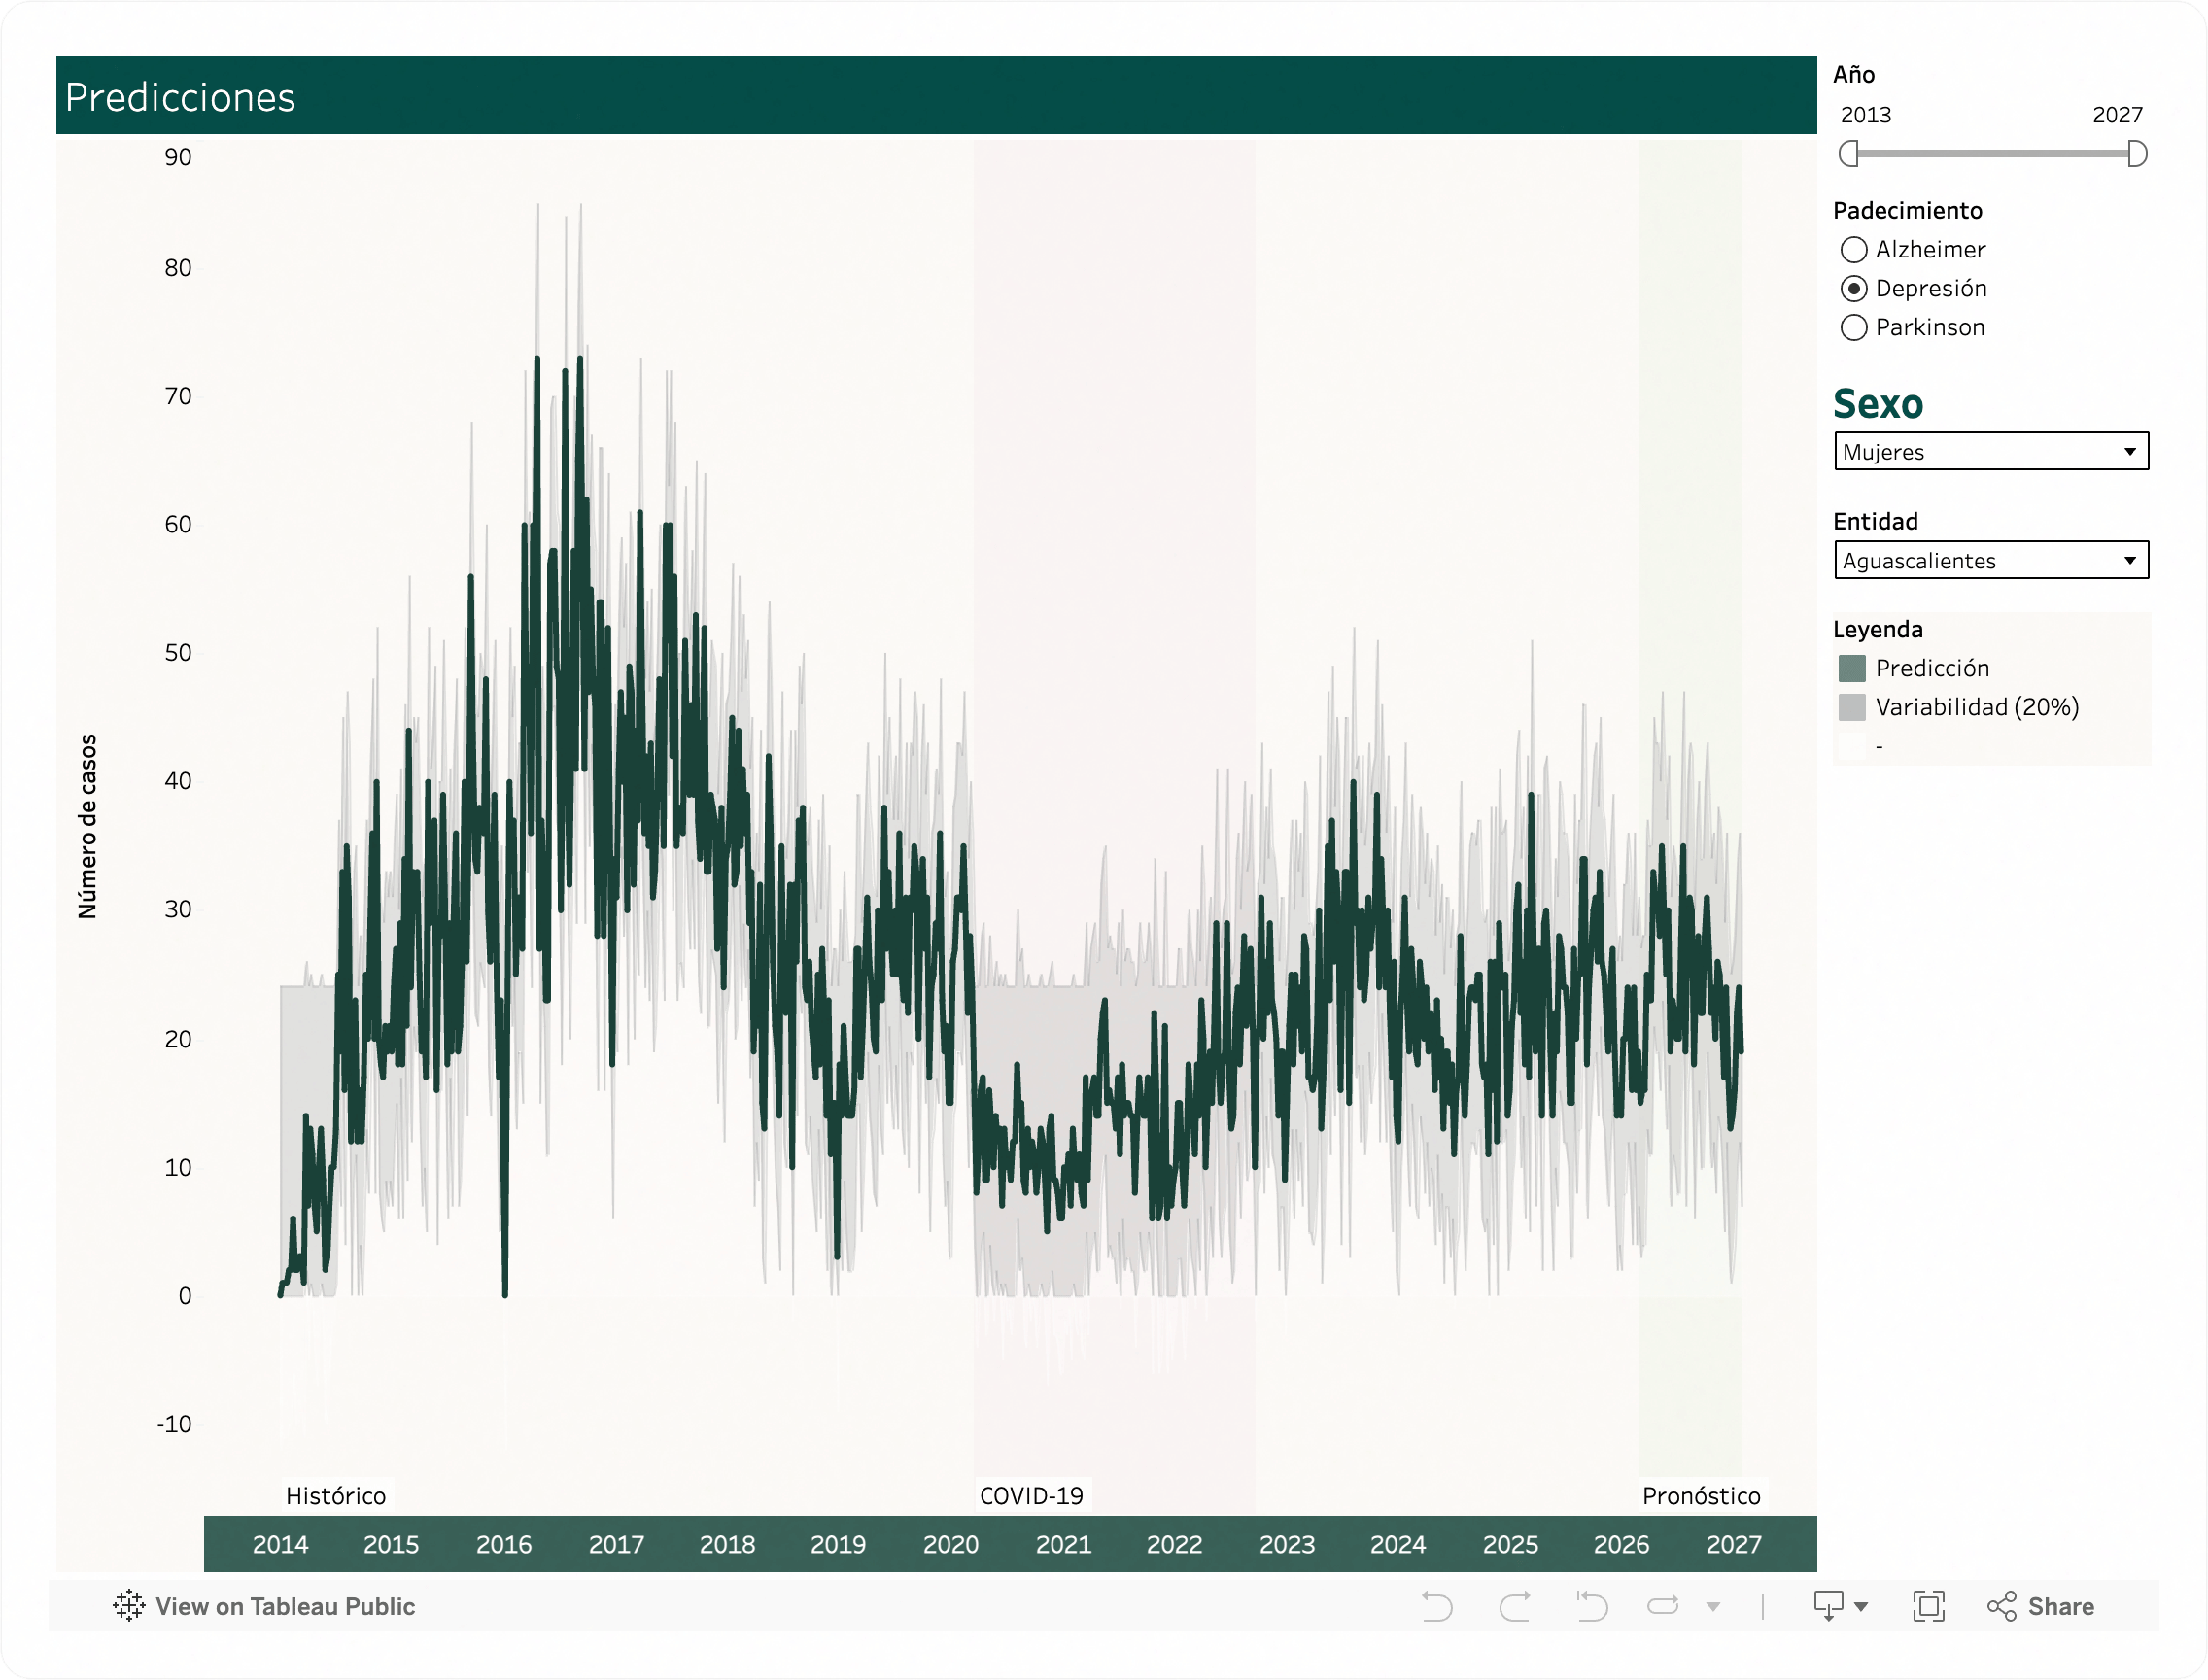
\includegraphics[width=\textwidth]{FigurasTableau/prediccion-estatal-banda.png}
\caption[Predicción estatal con banda de confianza.]{Vista de predicción \textbf{Predicción estatal con intervalo de confianza}: pronóstico a 52 semanas por entidad federativa con bandas al 80\% (\texttt{yhat\_lower} / \texttt{yhat\_upper}).}
\label{fig:web_prediccion_estatal_banda}
\end{figure}

\newpage
% -------------------------------------------------------------------------
% Predicción estatal
% -------------------------------------------------------------------------
La vista \textbf{Predicción estatal} presenta la serie histórica completa y el pronóstico a 52 semanas a nivel de entidad federativa, sin bandas de confianza, lo que facilita la lectura limpia de la tendencia proyectada. Es la versión simplificada de la vista anterior, diseñada para comunicar el pronóstico a perfiles no técnicos (coordinadores delegacionales, directivos regionales) que priorizan la claridad visual sobre el detalle estadístico. Los filtros disponibles son \textbf{padecimiento}, \textbf{entidad federativa} y \textbf{género}. La línea histórica y la línea de pronóstico se distinguen visualmente por color y la zona COVID-19 aparece sombreada para contextualizar el quiebre de tendencia observado en 2020--2022. El selector de entidad permite navegar entre las 32 entidades sin recargar el dashboard.

\begin{figure}[H]
\centering
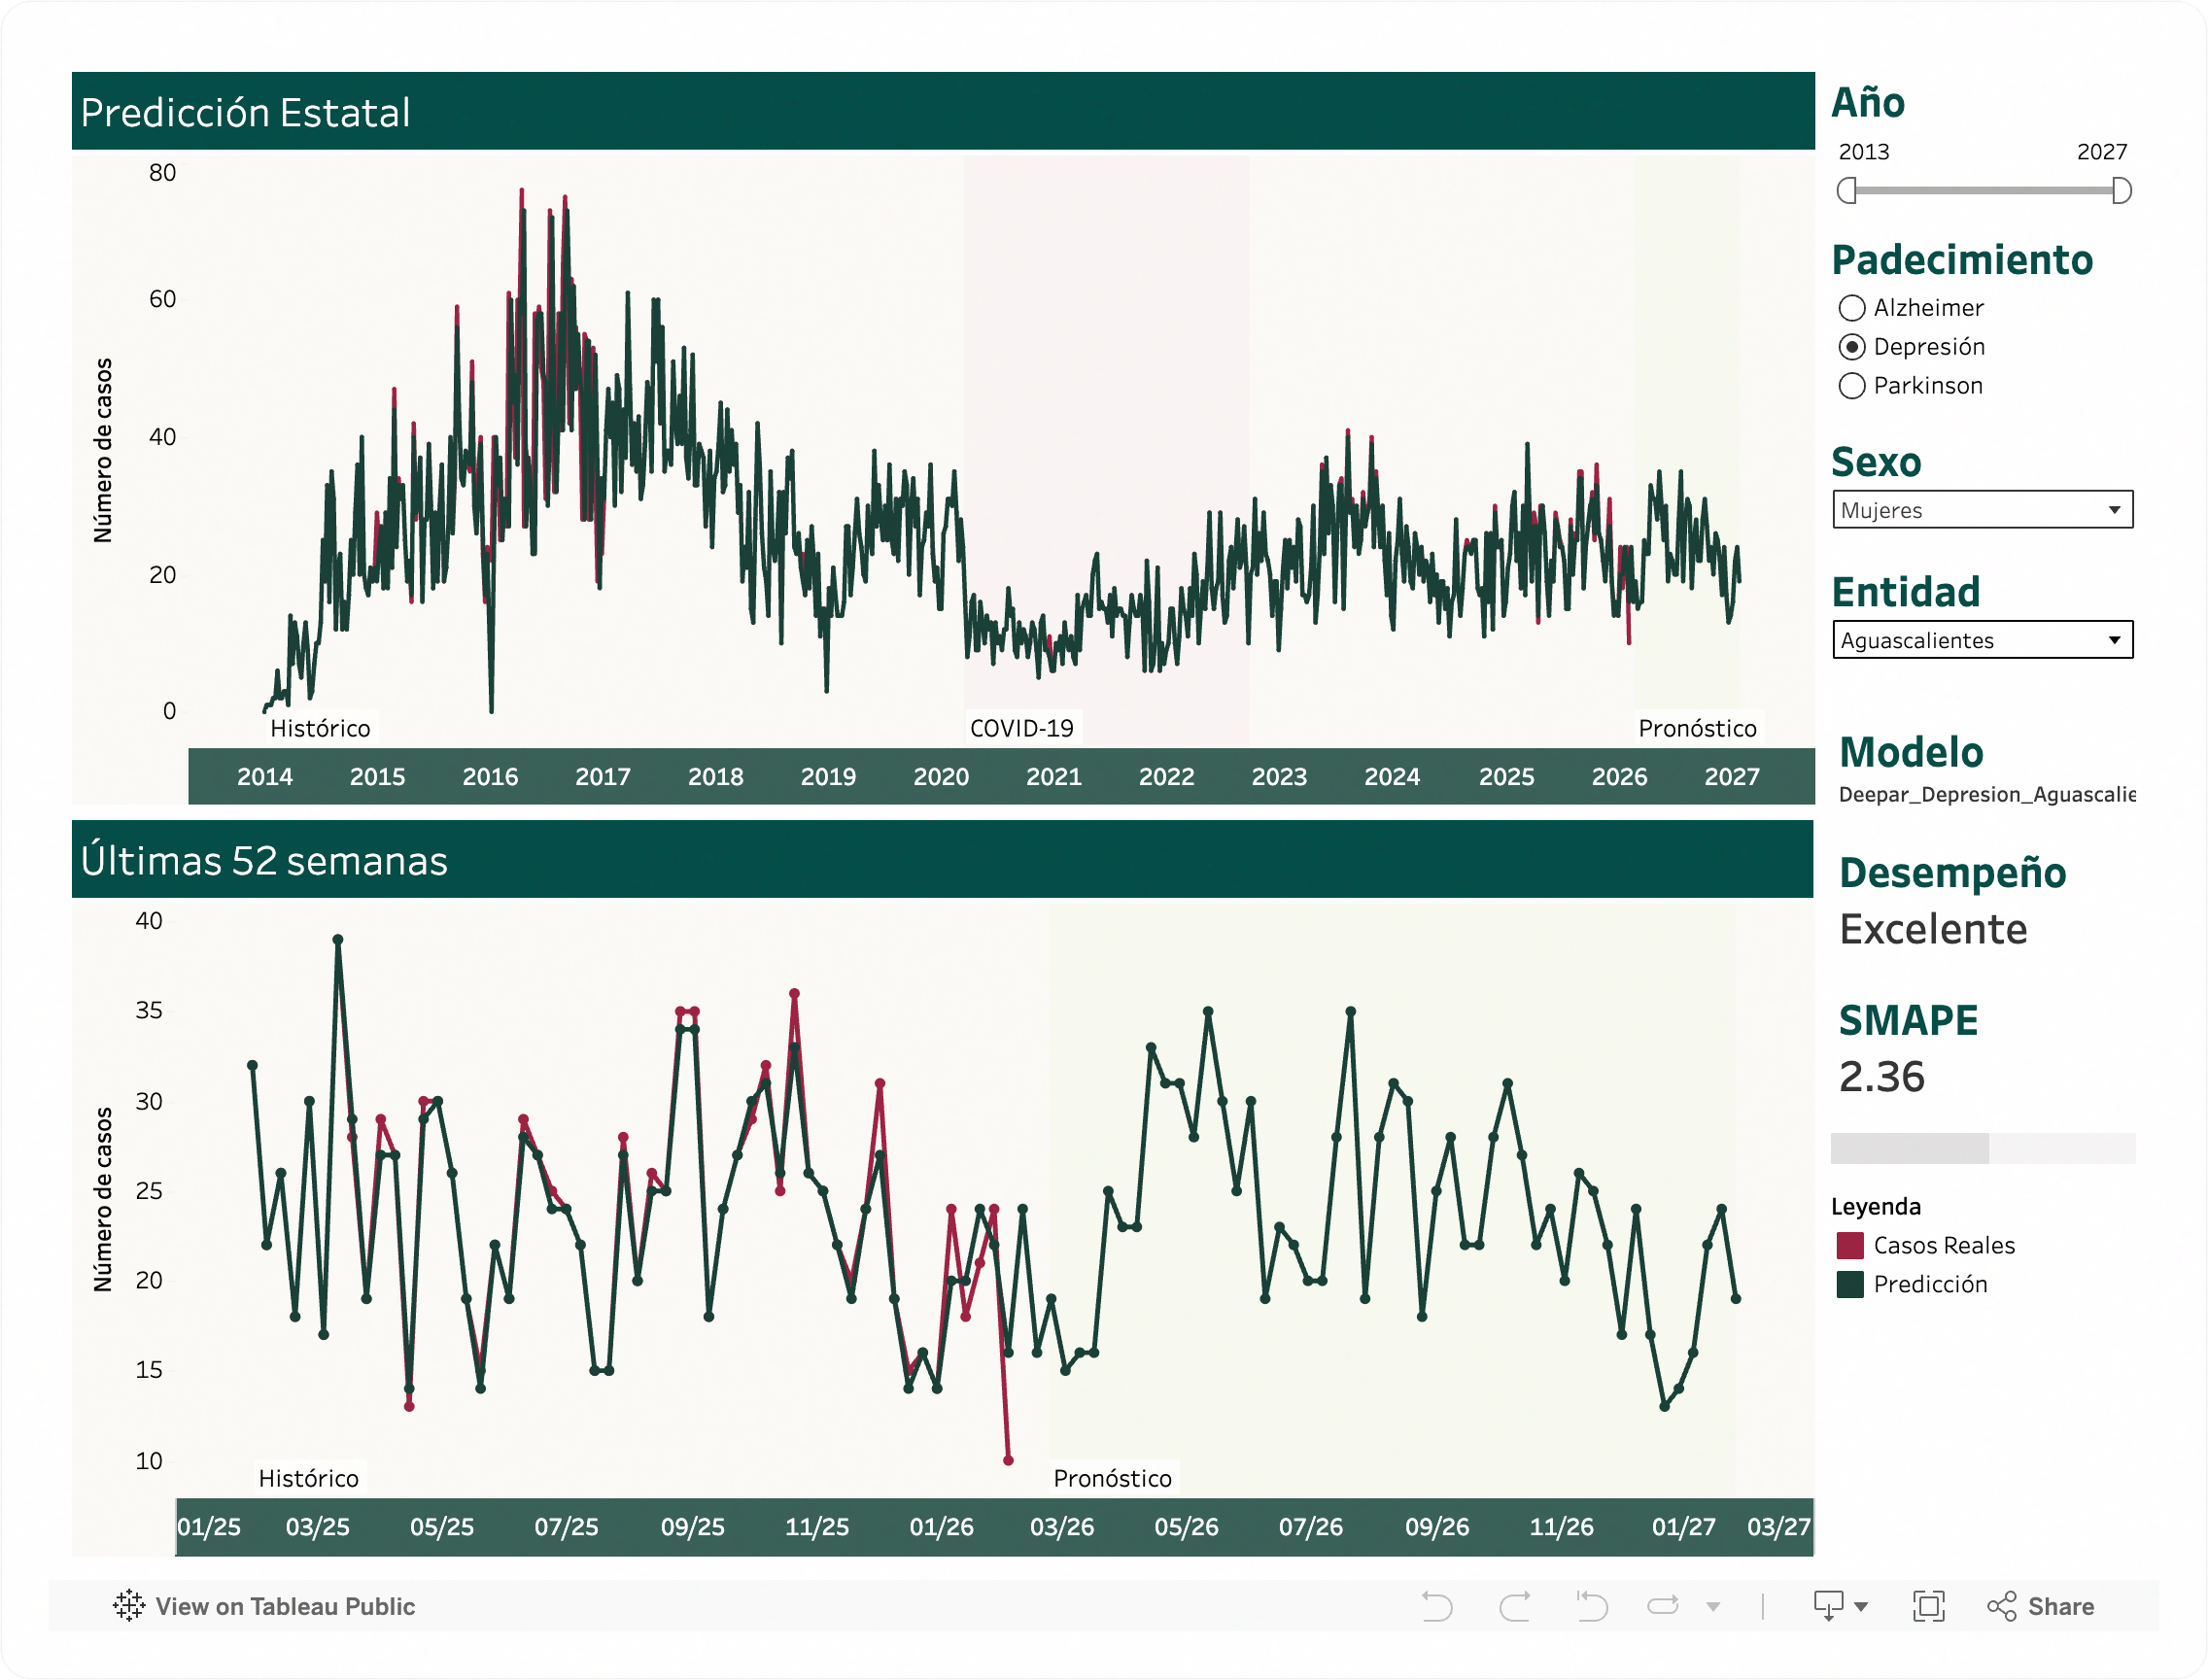
\includegraphics[width=\textwidth]{FigurasTableau/prediccion-estatal.png}
\caption[Predicción estatal.]{Vista de predicción \textbf{Predicción estatal}: serie histórica y pronóstico a 52 semanas a nivel de entidad federativa, con selector de estado, padecimiento y género.}
\label{fig:web_prediccion_estatal}
\end{figure}

\newpage
% -------------------------------------------------------------------------
% Predicción nacional
% -------------------------------------------------------------------------
La vista \textbf{Predicción nacional} es el punto de entrada principal del \textbf{DashNacional} y la interfaz de análisis de primer nivel para epidemiólogos de nivel federal. Muestra la serie temporal completa desde 2014 hasta 2027, integrando la serie histórica del \textsc{sinave}, el pronóstico a 52 semanas del modelo productivo seleccionado y la franja sombreada del periodo COVID-19 (marzo 2020 -- septiembre 2022). El panel lateral contextualiza el pronóstico con el \smape{} del modelo activo y una calificación cualitativa (Excelente / Bueno / Regular). Los filtros disponibles son \textbf{padecimiento} (Depresión, Parkinson, Alzheimer), \textbf{género} (General, Hombres, Mujeres) y \textbf{año}, lo que permite comparar visualmente el ajuste de distintos segmentos sobre la misma serie nacional. Esta vista es la recomendada para reuniones de planificación de recursos a nivel central del \textsc{imss}.

\begin{figure}[H]
\centering
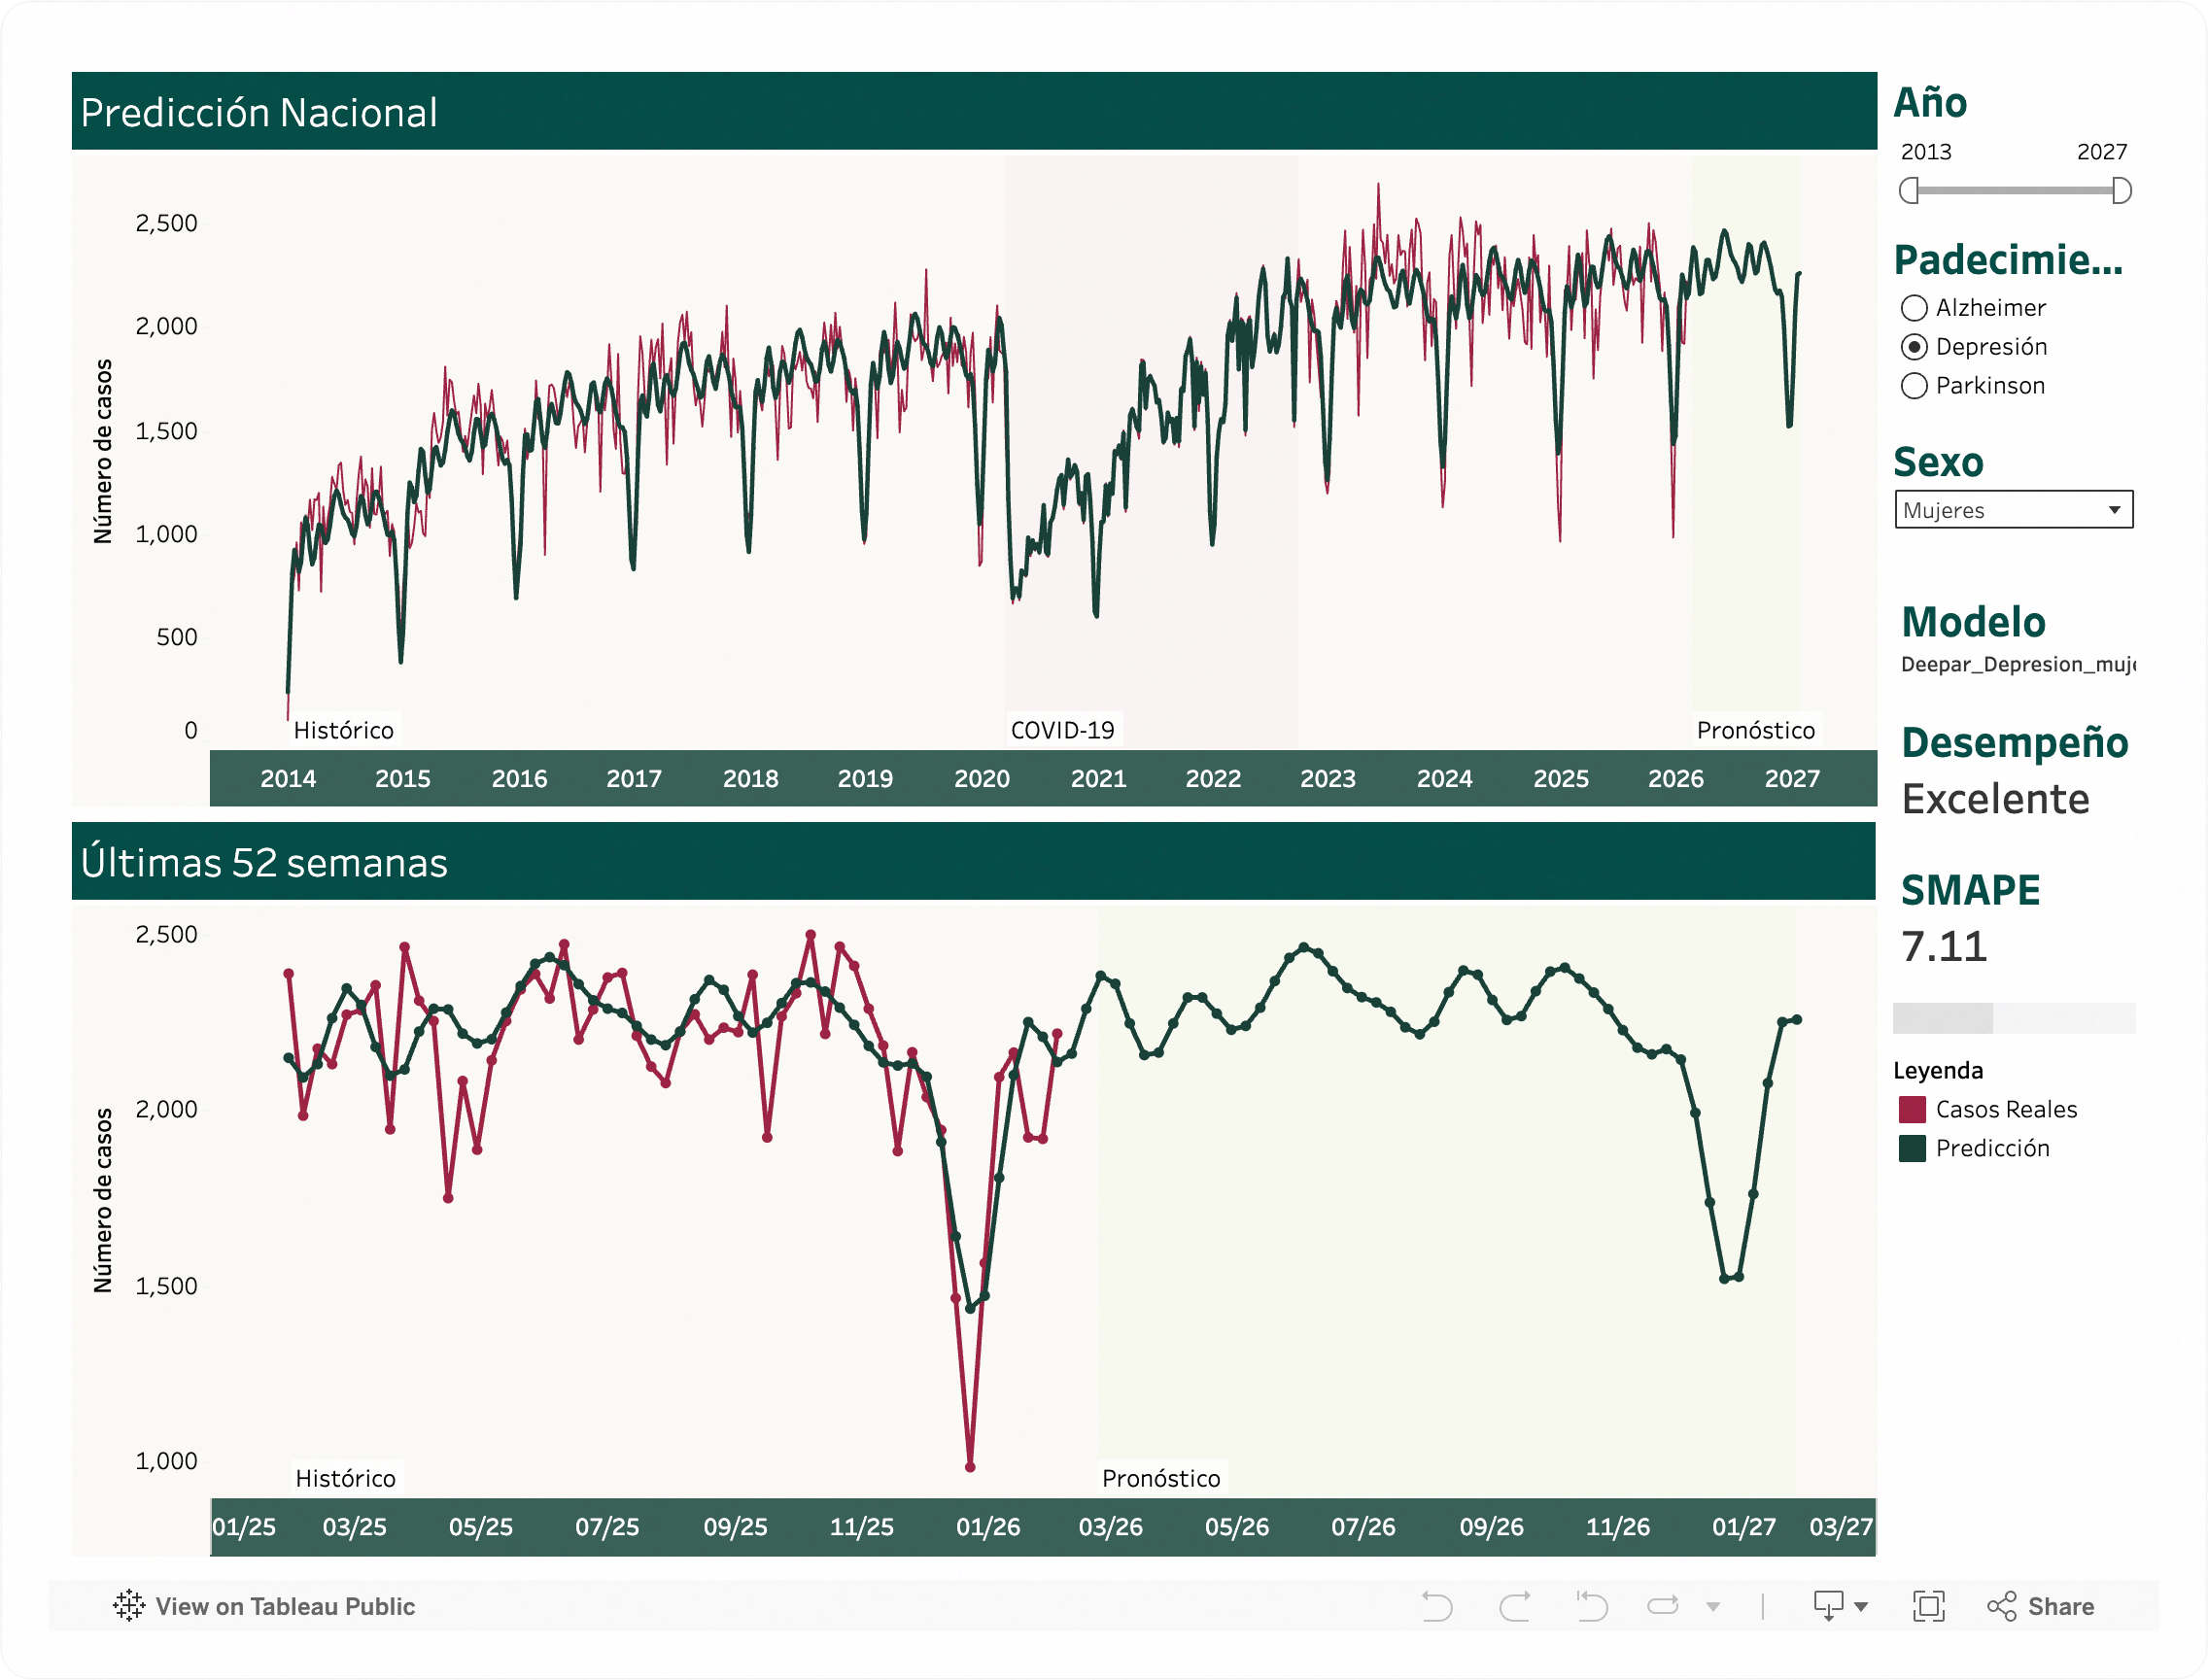
\includegraphics[width=\textwidth]{FigurasTableau/prediccion-nacional.png}
\caption[Predicción nacional.]{Vista de predicción \textbf{Predicción nacional}: serie temporal completa desde 2014 hasta 2027 con pronóstico a 52 semanas a nivel país, zona COVID-19 sombreada y métricas contextuales del modelo activo.}
\label{fig:web_prediccion_nacional}
\end{figure}

\newpage
% -------------------------------------------------------------------------
% Predicción regional
% -------------------------------------------------------------------------
La vista \textbf{Predicción regional} replica la lógica de la vista nacional pero a la escala de las cuatro regiones de salud mental construidas por el equipo a partir de indicadores del \textsc{inegi}: Metropolitana alta, Urbana media, Rural/dispersa y Sur-Sureste vulnerable. Permite comparar simultáneamente las tendencias y pronósticos de las cuatro regiones en un mismo eje, identificando divergencias macrorregionales que no serían visibles en la vista nacional agregada (por ejemplo, que la región Sur-Sureste vulnerable presenta una tendencia de Depresión más pronunciada que la región Metropolitana en el periodo post-COVID). Los filtros disponibles son \textbf{año}, \textbf{padecimiento} y \textbf{género}. Esta vista es especialmente útil para el análisis de inequidades territoriales en salud mental y para la planificación de intervenciones diferenciadas por región.

\begin{figure}[H]
\centering
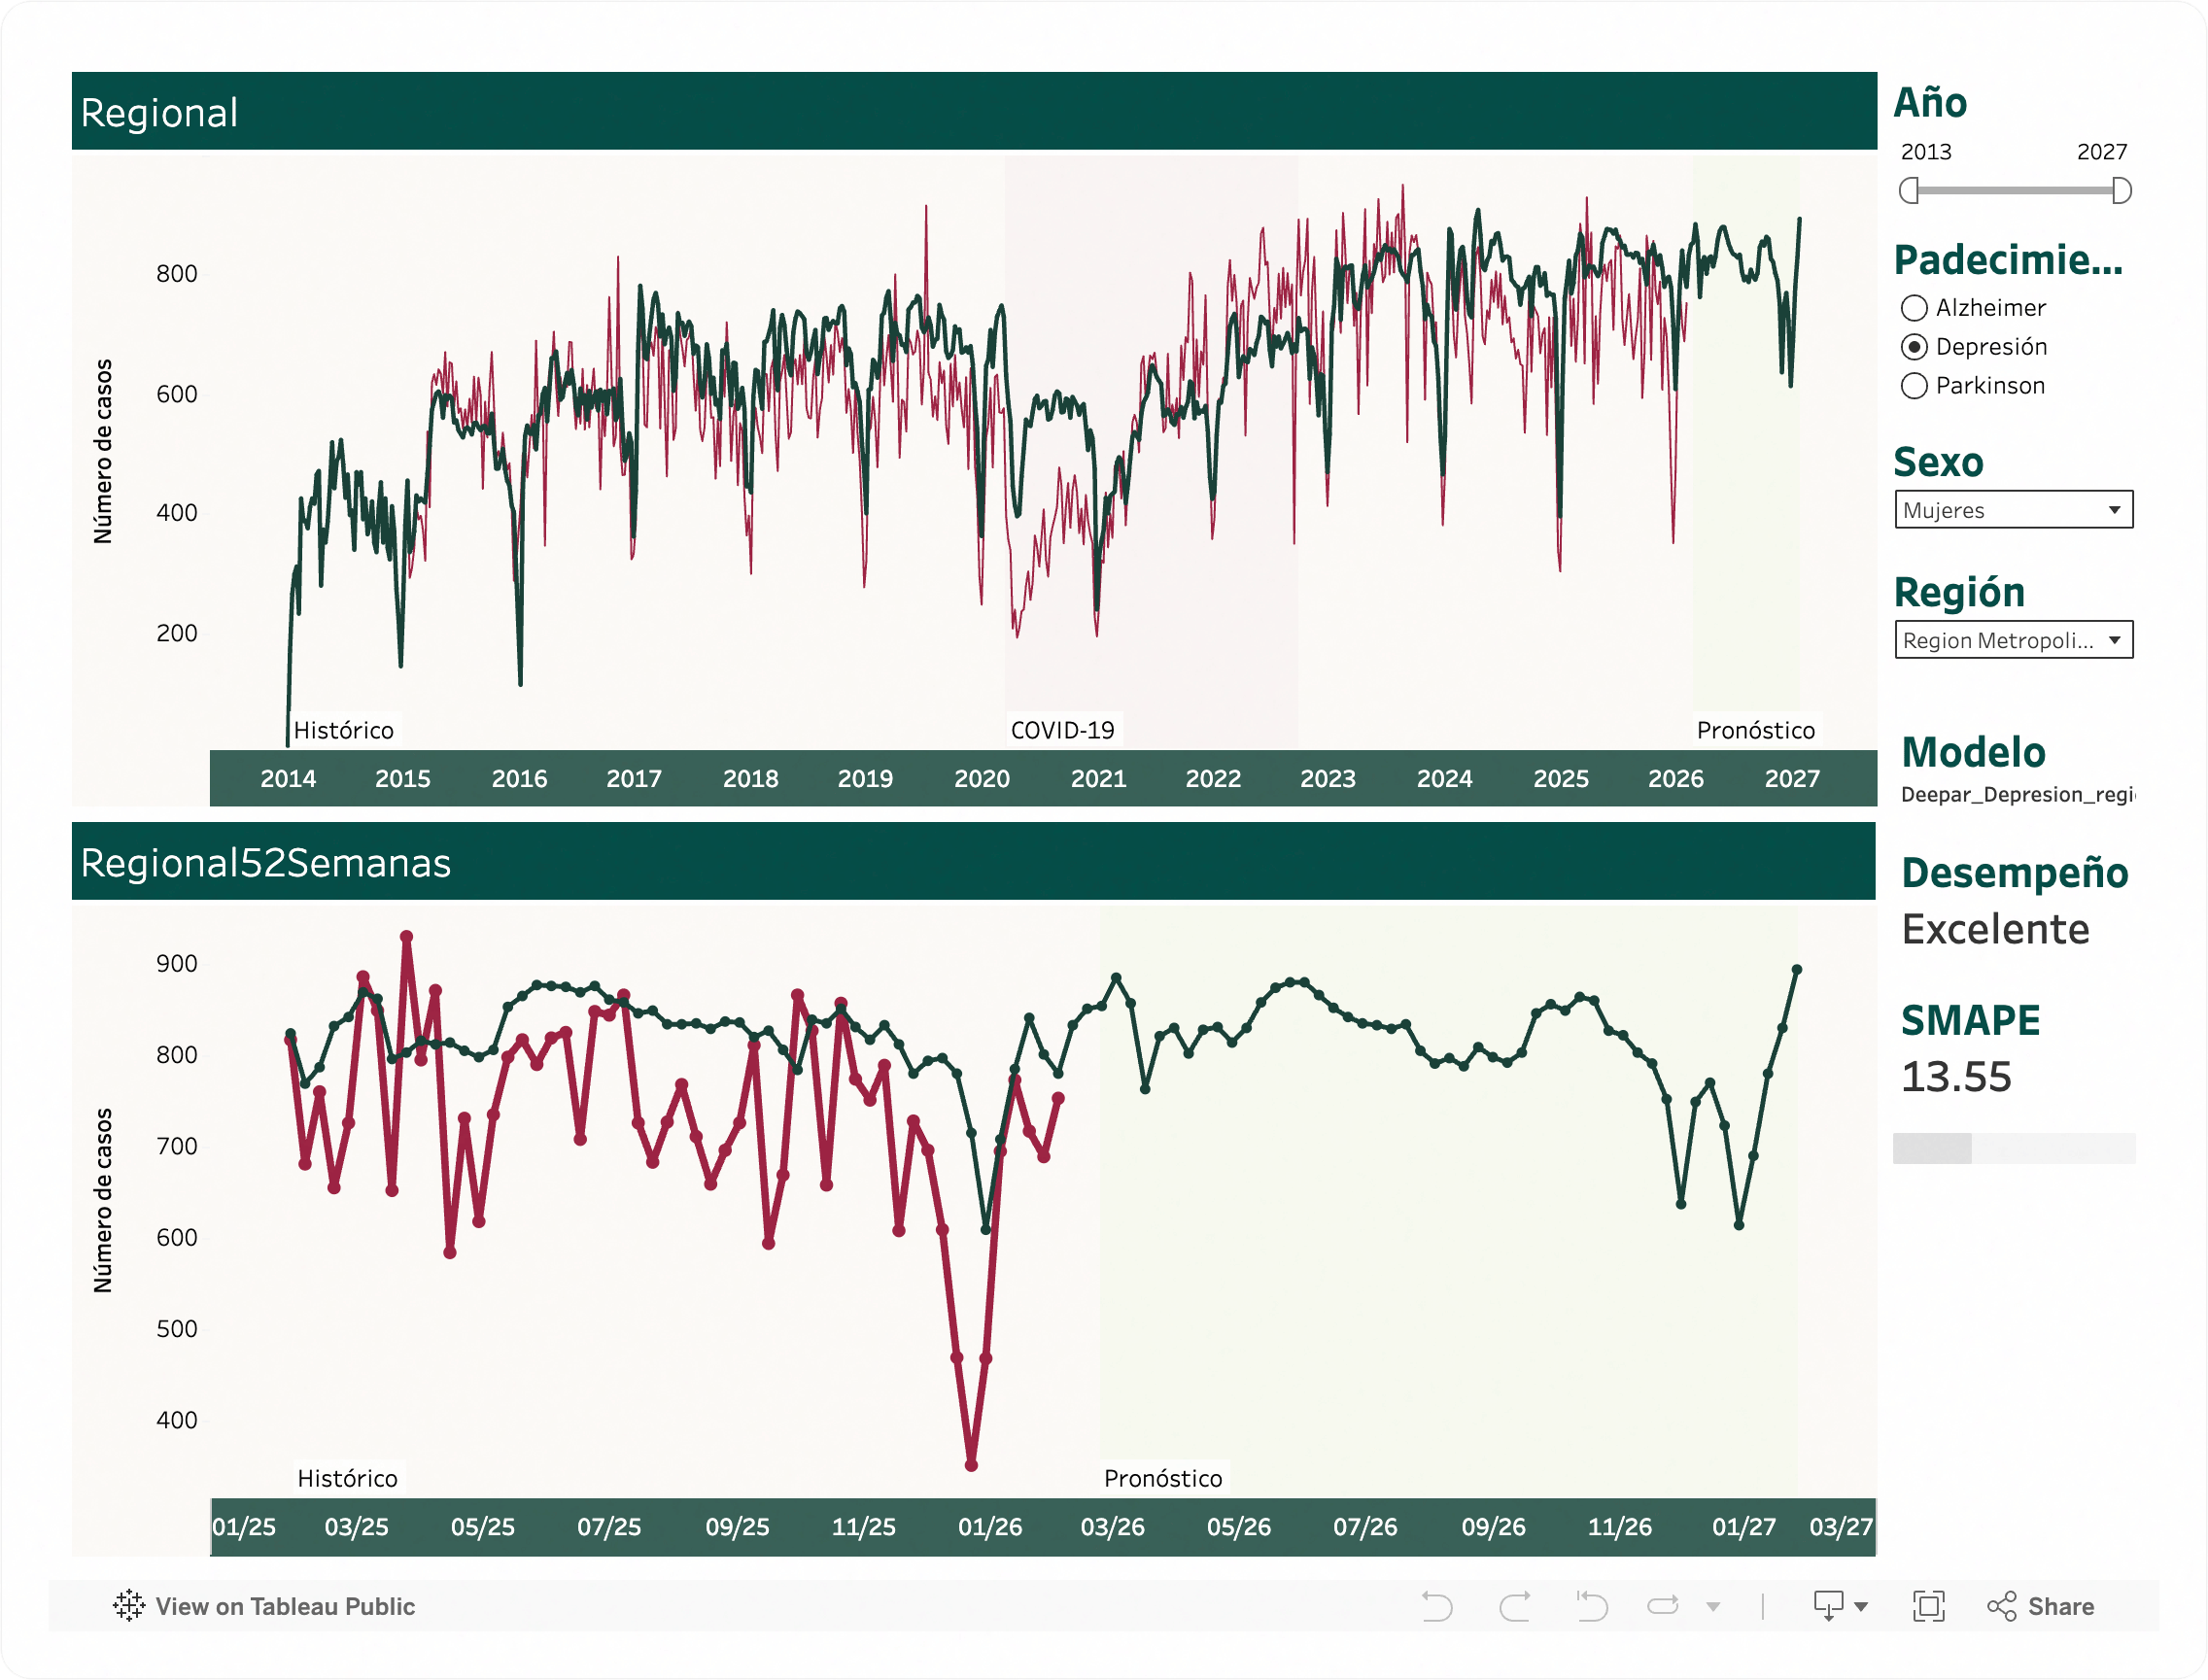
\includegraphics[width=\textwidth]{FigurasTableau/prediccion-regional.png}
\caption[Predicción regional.]{Vista de predicción \textbf{Predicción regional}: pronóstico agregado por las cuatro regiones de salud mental (Metropolitana alta, Urbana media, Rural/dispersa y Sur-Sureste vulnerable), con comparativa interregional.}
\label{fig:web_prediccion_regional}
\end{figure}

\newpage

% -------------------------------------------------------------------------
% DashKPIs
% -------------------------------------------------------------------------
El \textbf{DashKPIs} es la vista de control ejecutivo del sistema completo. Presenta en una sola pantalla los indicadores de salud del sistema de modelado: el total de modelos en producción (333), el número de modelos con desempeño excelente (\smape{} $<$ 15\%), la cobertura del sistema (100\%), y las métricas medianas globales (\smape{} = 23.66\%, \mase{} = 0.30). Incluye un \textit{heatmap} de métricas (\mae{}, \mape{}, \mase{}, \rmse{}, \smape{}) por padecimiento, nivel geográfico y género; un donut chart con la distribución de algoritmos activos (DeepAR, Prophet, Ensemble, Stacking); y una grilla de calor por serie que permite identificar qué motor está asignado a cada combinación de padecimiento, entidad y género. Esta vista está diseñada como punto de entrada para directivos y para el equipo técnico en tareas de monitoreo. No requiere filtros para su interpretación inicial, aunque los filtros de padecimiento y género están disponibles y sincronizados con el resto del workbook.

\begin{figure}[H]
\centering
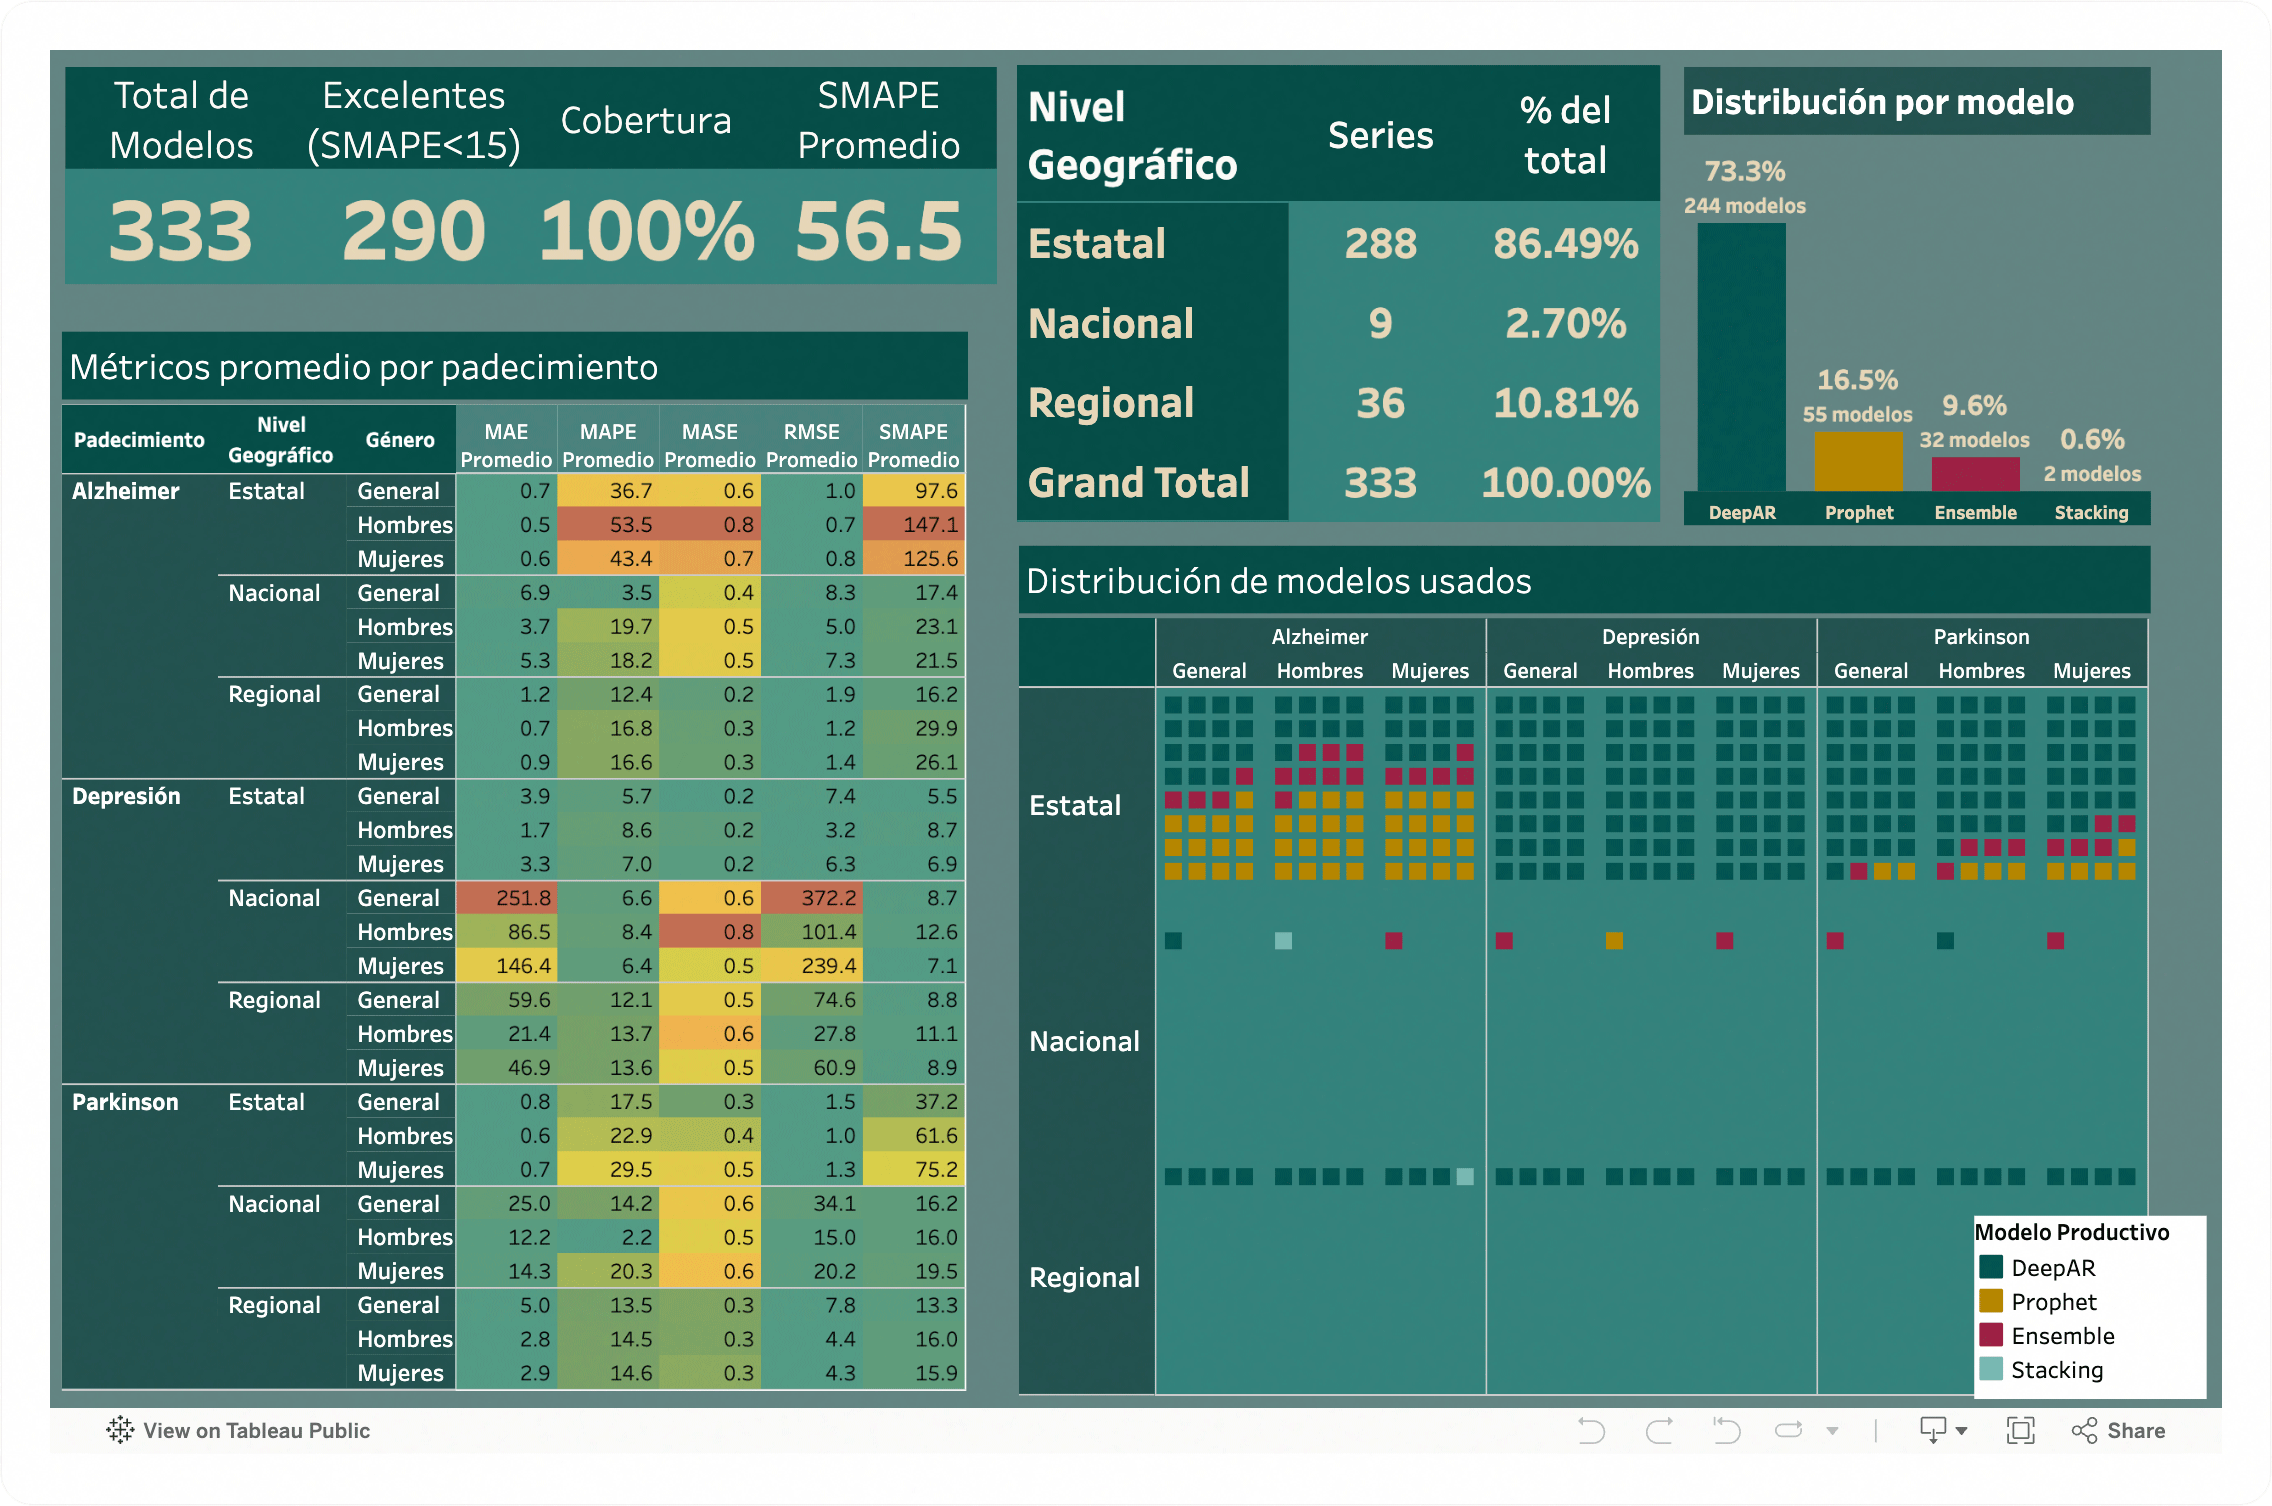
\includegraphics[width=0.85\textwidth]{FigurasTableau/dashboard-kpis}
\caption[Dashboard KPIs — Monitoreo del sistema de modelado.]{Vista \textbf{DashKPIs}: indicadores generales del sistema de pronóstico, distribución de algoritmos en producción, heatmap de métricas y mapa de calor por serie.}
\label{fig:web_dashboard_kpis}
\end{figure}

\newpage

% =============================================================================
% 9. VARIABLES Y MÉTRICAS DEL SISTEMA
% =============================================================================
\section{Variables y Métricas del Sistema}\label{sec:variables}

\subsection{Inventario completo de variables}

\begin{table}[H]
\centering
\caption{Variables temporales y epidemiológicas}
\label{tab:vars_epid}
\small
\begin{tabularx}{\textwidth}{>{\ttfamily}l l X}
\toprule
\textbf{Variable} & \textbf{Tabla} & \textbf{Descripción} \\
\midrule
ds               & scaffold, real, forecast & Fecha epidemiológica (\texttt{YYYY-MM-DD}); índice temporal. \\
padecimiento     & scaffold              & Enfermedad: Depresión (F32), Parkinson (G20), Alzheimer (G30). \\
entidad          & scaffold, entidades   & Entidad federativa, región o nivel Nacional. \\
genero           & scaffold, metricas    & Estrategia: \texttt{general}, \texttt{hombres}, \texttt{mujeres}. \\
incrementos\_total   & real             & Casos observados totales (ambos géneros). \\
incrementos\_hombres & real             & Casos observados en hombres. \\
incrementos\_mujeres & real             & Casos observadas en mujeres. \\
yhat             & forecast              & Pronóstico del modelo productivo (entero redondeado). \\
yhat\_lower      & forecast              & Límite inferior del intervalo de confianza al 80\%. \\
yhat\_upper      & forecast              & Límite superior del intervalo de confianza al 80\%. \\
modelo\_productivo & metricas            & Algoritmo ganador: \texttt{deepar}, \texttt{prophet}, \texttt{ensemble}, \texttt{stacking}. \\
\bottomrule
\end{tabularx}
\end{table}

\begin{table}[H]
\centering
\caption{Variables demográficas y territoriales (tabla \texttt{entidades})}
\label{tab:vars_demo}
\small
\begin{tabularx}{\textwidth}{>{\ttfamily}l X}
\toprule
\textbf{Variable} & \textbf{Descripción} \\
\midrule
Region                          & Región geográfica del país (Norte, Centro, Sur, etc.). \\
Region Socio-Urbana             & Clasificación territorial socioeconómica (Metropolitana alta, Urbana media, Rural/dispersa, Sur-Sureste vulnerable). \\
Superficie\_km2                 & Extensión territorial de la entidad federativa en km$^2$. \\
densidad\_poblacion             & Densidad poblacional (habitantes/km$^2$). \\
densidad\_poblacional\_percentil & Clasificación relativa de densidad (percentil). \\
extension\_territorial\_percentil & Clasificación relativa de superficie (percentil). \\
tamano\_poblacional\_predefinido & Categoría de tamaño poblacional predefinida. \\
ratio\_h\_m\_cat                & Categoría de la relación hombres-mujeres. \\
Poblacion Hombres               & Población masculina total de la entidad. \\
Poblacion Mujeres               & Población femenina total de la entidad. \\
\bottomrule
\end{tabularx}
\end{table}

\subsection{Métricas de desempeño de los modelos}

\begin{table}[H]
\centering
\caption{Métricas de evaluación de modelos de pronóstico}
\label{tab:metricas}
\small
\begin{tabularx}{\textwidth}{l X l}
\toprule
\textbf{Métrica} & \textbf{Descripción} & \textbf{Interpretación} \\
\midrule
\smape{} & Symmetric Mean Absolute Percentage Error. Error porcentual simétrico; rango $[0\%, 200\%]$. & Menor es mejor. \\
\mase{}  & Mean Absolute Scaled Error. Error comparado contra el modelo naive estacional (lag-52). & $<$1 supera al naive. \\
\rmse{}  & Root Mean Squared Error. Penaliza errores grandes; en unidades del caso. & Menor es mejor. \\
\mae{}   & Mean Absolute Error. Error promedio absoluto; robusto a valores extremos. & Menor es mejor. \\
\mape{}  & Mean Absolute Percentage Error. Error porcentual asimétrico; distorsionado cuando los valores reales son cercanos a cero. & Referencial. \\
\bottomrule
\end{tabularx}
\end{table}

\begin{warningbox}[Limitación del \smape{} en series de baja incidencia]
Para series con incidencia semanal menor a 5 casos (frecuente en Alzheimer y Parkinson en estados pequeños), el \smape{} puede superar el 100\% aunque el error absoluto sea menor a 1 caso por semana. En estos casos, el \mae{} y el \rmse{} son métricas más informativas sobre la utilidad clínica del modelo.
\end{warningbox}

\newpage
% =============================================================================
% 10. INTEGRACIÓN CON GOOGLE SHEETS
% =============================================================================
\section{Integración con Google Sheets}\label{sec:gsheets}

\subsection{Script \texttt{publish\_gsheets.py}}

El script \texttt{publish\_gsheets.py} es responsable de publicar el dataset de Tableau en Google Sheets. Opera de la siguiente manera:

\begin{enumerate}[noitemsep]
    \item Lee \texttt{tableau\_model.xlsx} y carga las cinco hojas en memoria como DataFrames de pandas.
    \item Convierte las columnas de tipo \texttt{datetime} a cadenas \texttt{YYYY-MM-DD}, ya que la API de Google Sheets no acepta objetos Timestamp en la serialización JSON.
    \item Imprime un resumen de filas, columnas y celdas por tabla antes de iniciar la publicación.
    \item Autentica contra la API de Google Sheets mediante una cuenta de servicio GCP.
    \item Para cada tabla: redimensiona la hoja si es necesario, borra su contenido actual, escribe la cabecera y escribe los datos en bloques de 5,000 filas con reporte de progreso cada 10 puntos porcentuales.
    \item Elimina pestañas del esquema anterior (\texttt{tableau\_1}, \texttt{tableau\_2}, \ldots) si aún existen.
    \item Actualiza la pestaña \texttt{meta} con el timestamp de publicación y el resumen de volumen.
\end{enumerate}

\subsection{Autenticación y secretos}

La autenticación utiliza una cuenta de servicio de Google Cloud Platform. Las credenciales se almacenan como secretos en el repositorio de GitHub y se inyectan como variables de entorno en el job de CI/CD:

\begin{table}[H]
\centering
\caption{Secretos y variables de configuración}
\label{tab:secretos}
\small
\begin{tabularx}{\textwidth}{>{\ttfamily}l l X}
\toprule
\textbf{Nombre} & \textbf{Tipo} & \textbf{Descripción} \\
\midrule
GOOGLE\_SERVICE\_ACCOUNT\_JSON & GitHub Secret   & JSON completo de la cuenta de servicio GCP. \\
GSHEETS\_SPREADSHEET\_ID       & GitHub Variable & ID del Google Sheet de destino. \\
GSHEETS\_CHUNK\_SIZE           & Env variable    & Tamaño de bloque de escritura (default: 5,000 filas). \\
\bottomrule
\end{tabularx}
\end{table}

\subsection{Google Sheets como fuente de datos para Tableau Public}

La razón de usar Google Sheets como intermediario (en lugar de publicar directamente desde S3 o un archivo local) es que Tableau Public soporta actualizaciones automáticas del \textit{extract} desde Google Sheets. Cuando el script publica una nueva versión del dataset, Tableau Public detecta el cambio y refresca el extract de forma automática en un ciclo de aproximadamente 24 horas, propagando las actualizaciones a las visualizaciones embebidas en el sitio web sin intervención manual.

\newpage
% =============================================================================
% 11. AUTOMATIZACIÓN CON GITHUB ACTIONS
% =============================================================================
\section{Automatización con GitHub Actions}\label{sec:ci}

\subsection{Workflow \texttt{gsheets.yml}}

El proceso de publicación está completamente automatizado mediante un workflow de GitHub Actions definido en \texttt{.github/workflows/gsheets.yml}. El workflow puede dispararse de dos formas:

\begin{itemize}[noitemsep]
    \item \textbf{\texttt{workflow\_call}}: invocado automáticamente desde otro workflow cuando el pipeline de datos genera un nuevo \texttt{tableau\_model.xlsx}.
    \item \textbf{\texttt{workflow\_dispatch}}: ejecución manual desde la interfaz de GitHub, útil para forzar una republicación sin cambios en los datos.
\end{itemize}

\subsection{Pasos del job de publicación}

\begin{enumerate}[noitemsep]
    \item \textbf{Checkout}: descarga el código fuente del repositorio incluyendo \texttt{tableau\_model.xlsx}.
    \item \textbf{Setup Python 3.12}: configura el entorno de ejecución.
    \item \textbf{Instalación de dependencias}: instala el paquete \texttt{epiforecast} con extras de Google Sheets (\texttt{pip install -e ".[gsheets]"}).
    \item \textbf{Publicación}: ejecuta \texttt{python -m scripts.publish\_gsheets} con las variables de entorno inyectadas desde los secretos del repositorio.
\end{enumerate}

\subsection{Trabajo futuro: publicación incremental}

Actualmente el script publica el dataset completo en cada ejecución, lo que implica reescribir las $\sim$2.4 millones de celdas cada vez. Se está explorando una estrategia de publicación incremental que detecte únicamente las filas nuevas (por comparación del campo \texttt{ds} con la última fecha publicada en la pestaña \texttt{meta}) y las agregue sin reescribir el dataset completo. Esta mejora reduciría el tiempo de publicación de $\sim$8 minutos a menos de 1 minuto para actualizaciones semanales rutinarias.

\newpage
% =============================================================================
% 12. PROCESO DE PUBLICACIÓN DEL DASHBOARD
% =============================================================================
\section{Proceso de Publicación del Dashboard}\label{sec:publicacion}

El proceso completo de despliegue, desde la generación del dataset hasta la actualización de las visualizaciones en el sitio web, sigue la siguiente secuencia:

\begin{enumerate}[noitemsep]
    \item \textbf{Generación del dataset}: \texttt{make tableau} ejecuta \texttt{build\_tableau.py} y produce \texttt{tableau\_model.xlsx} con las cinco hojas normalizadas.
    \item \textbf{Publicación de los datos}: Al disparar el workflow \texttt{gsheets.yml}, ya sea manual o automáticamente, se publican las cinco hojas en el Google Sheet de destino.
    \item \textbf{Refresco del extract}: Tableau Public toma la información actualizada desde Google Sheets y actualiza el extract en un ciclo de $\sim$24 horas.
    \item \textbf{Actualización de las visualizaciones}: el embed code embebido en \url{https://proyectointegrador.org/epidashboard} sirve automáticamente la versión más reciente del dashboard sin modificación del sitio web.
\end{enumerate}

El estado actual del sistema es: pipeline finalizado, \texttt{tableau\_model.xlsx} publicado, dashboard activo en Tableau Public y visualizaciones embebidas en el sitio web.

\newpage
% =============================================================================
% 13. DECISIONES TÉCNICAS DE DISEÑO
% =============================================================================
\section{Decisiones Técnicas de Diseño}\label{sec:decisiones}

\begin{table}[H]
\centering
\caption{Decisiones técnicas relevantes y su justificación}
\label{tab:decisiones}
\scriptsize
\setlength{\tabcolsep}{4pt}
\begin{tabularx}{\textwidth}{>{\bfseries}p{3.2cm} X X}
\toprule
\textbf{Decisión} & \textbf{Descripción} & \textbf{Justificación} \\
\midrule
Normalización por 100,000 habitantes & Las visualizaciones de \textit{Casos por año} y \textit{Casos por semana} normalizan la incidencia por población. & Permite comparar entidades con poblaciones muy diferentes (Ciudad de México vs.\ Colima) en el mismo eje. \\
\addlinespace
Recorte por percentiles & Las vistas de evolución aplican un límite superior basado en percentiles del eje Y. & Evita que outliers temporales (como el rebote post-COVID de Depresión) distorsionen la escala de la gráfica para el resto de la serie. \\
\addlinespace
Exclusión de agregados en filtros de entidad & Los filtros de entidad no incluyen por defecto las filas de nivel Nacional ni regional. & Evita doble conteo cuando el usuario quiere explorar la suma de estados. Los niveles Nacional y Regional tienen sus propias vistas dedicadas. \\
\addlinespace
\texttt{scaffold} como ancla central & El modelo relacional usa \texttt{scaffold} como tabla raíz en lugar de \texttt{forecast} o \texttt{real}. & Garantiza que los filtros interactivos se propaguen simultáneamente a ambas tablas de hechos (véase \secref{sec:modelo_relacional}). \\
\addlinespace
\texttt{yhat} redondeado a entero & Los pronósticos se publican como \texttt{Int64}, no como \texttt{float}. & Los casos son conteos discretos; mostrar decimales como ``14.3 casos'' carecería de significado clínico. \\
\addlinespace
Relationships en lugar de joins físicos & El modelo de Tableau usa \textit{relationships} (modelo lógico) en lugar de \texttt{JOIN} SQL. & Evita la multiplicación de filas al relacionar tablas con cardinalidades diferentes; Tableau ejecuta los joins en tiempo de consulta solo para los campos que se necesitan. \\
\bottomrule
\end{tabularx}
\end{table}

\newpage
% =============================================================================
% 14. CONCLUSIONES
% =============================================================================
\section{Conclusiones}\label{sec:conclusiones}

El sistema de visualización epidemiológica implementado en \texttt{viz\_epiforecastmx.twb} representa una plataforma integral que transforma datos epidemiológicos complejos en información accionable para la toma de decisiones clínicas y administrativas dentro del {\imss}.

Desde el punto de vista técnico, la migración del diseño plano (\texttt{tableau.csv}) al modelo relacional normalizado (\texttt{tableau\_model.xlsx}) fue la decisión de arquitectura más significativa del proyecto: resolvió simultáneamente el límite de volumen de Google Sheets, el problema de propagación de filtros en Tableau y la duplicación de datos demográficos por fecha. La tabla \texttt{scaffold} como ancla central es el mecanismo clave que permite que un solo filtro interactivo controle tanto la serie histórica como el pronóstico en todas las vistas del workbook.

La automatización completa mediante GitHub Actions garantiza que el ciclo de actualización del dashboard sea reproducible y no dependa de intervenciones manuales: cualquier miembro del equipo puede publicar una nueva versión del dataset ejecutando \texttt{make tableau} seguido de un push al repositorio, y el dashboard en el sitio web se actualizará automáticamente en las siguientes 24 horas.

El valor clínico del sistema reside en tres capacidades concretas: la posibilidad de explorar tendencias epidemiológicas a cualquier nivel de granularidad geográfica (nacional, regional, estatal), la disponibilidad de pronósticos a 52 semanas con intervalos de confianza para anticipar la demanda de recursos, y el monitoreo del desempeño del sistema de modelado mediante KPIs que permiten detectar degradación antes de que afecte la calidad de los pronósticos.

Como trabajo futuro inmediato, la implementación de publicación incremental en \texttt{publish\_gsheets.py} reducirá significativamente el tiempo del ciclo de actualización semanal.

\vspace{1.0cm}
\begin{center}
\textcolor{coolgray}{\rule{0.5\textwidth}{0.4pt}}\\[0.3cm]
{\small\textcolor{coolgray}{Documentación técnica del Sistema de Visualización Tableau}}\\
{\small\textcolor{coolgray}{Proyecto EpiForecast-MX | TC5035.10}}\\
{\small\textcolor{coolgray}{Maestría en Inteligencia Artificial Aplicada, Tecnológico de Monterrey}}\\
{\small\textcolor{coolgray}{Marzo 2026}}
\end{center}

\end{document}
